\documentclass[12pt, openany]{report}
\usepackage[utf8]{inputenc}
\usepackage[T1]{fontenc}
\usepackage{amsmath,amsfonts,amssymb}
\usepackage{amssymb}
\usepackage{multicol}
\usepackage[a4paper,left=2.5cm,right=2.5cm,top=2.5cm,bottom=2.5cm]{geometry}
\usepackage[english]{babel}
\usepackage{libertine}
\usepackage{graphicx}
\usepackage{wrapfig}
\usepackage{algorithm}
\usepackage{algpseudocode}
\usepackage{float}
\usepackage{enumitem}
\usepackage{pythonhighlight}
\usepackage[]{titletoc}
\usepackage{empheq}
\usepackage{titlesec}
\usepackage{mathpazo}
\usepackage{xfrac}
\usepackage{textcomp}
\usepackage{mathtools}
\usepackage{caption}
\usepackage{tabularray}
\usepackage{subcaption}
\usepackage[bottom]{footmisc}
\usepackage{pdfpages}
\usepackage{tabularx}
\usepackage{amsthm}
\usepackage{listings}
\usepackage[skins]{tcolorbox}
\titleformat{\chapter}[display]
  {\normalfont\bfseries}{}{0pt}{\Huge}
\usepackage{hyperref}
\newcommand{\hsp}{\hspace{20pt}}
\newcommand{\HRule}{\rule{\linewidth}{0.5mm}}
\newcommand{\R}{\mathbb{R}}
\newcommand{\C}{\mathbb{C}}
\theoremstyle{definition}
\newtheorem{thm}{Theorem}[chapter]
\newtheorem{definition}[thm]{Definition}
\newtheorem{lem}[thm]{Lemma}


\definecolor{mGreen}{rgb}{0,0.6,0}
\definecolor{mGray}{rgb}{0.5,0.5,0.5}
\definecolor{mPurple}{rgb}{0.58,0,0.82}
\definecolor{backgroundColour}{rgb}{0.95,0.95,0.92}
\definecolor{light-gray}{gray}{0.95}
\newcommand{\code}[1]{\colorbox{light-gray}{\texttt{#1}}}

\lstdefinestyle{CppStyle}{
    backgroundcolor=\color{backgroundColour},   
    commentstyle=\color{mGreen},
    keywordstyle=\color{magenta},
    numberstyle=\tiny\color{mGray},
    stringstyle=\color{mPurple},
    basicstyle=\footnotesize,
    breakatwhitespace=false,         
    breaklines=true,                 
    captionpos=b,                    
    keepspaces=true,                 
    numbers=left,                    
    numbersep=5pt,                  
    showspaces=false,                
    showstringspaces=false,
    showtabs=false,                  
    tabsize=2,
    language=C
}

\hbadness=100000
\begin{document}
\begin{titlepage}
    \begin{sffamily}
    \begin{center}
        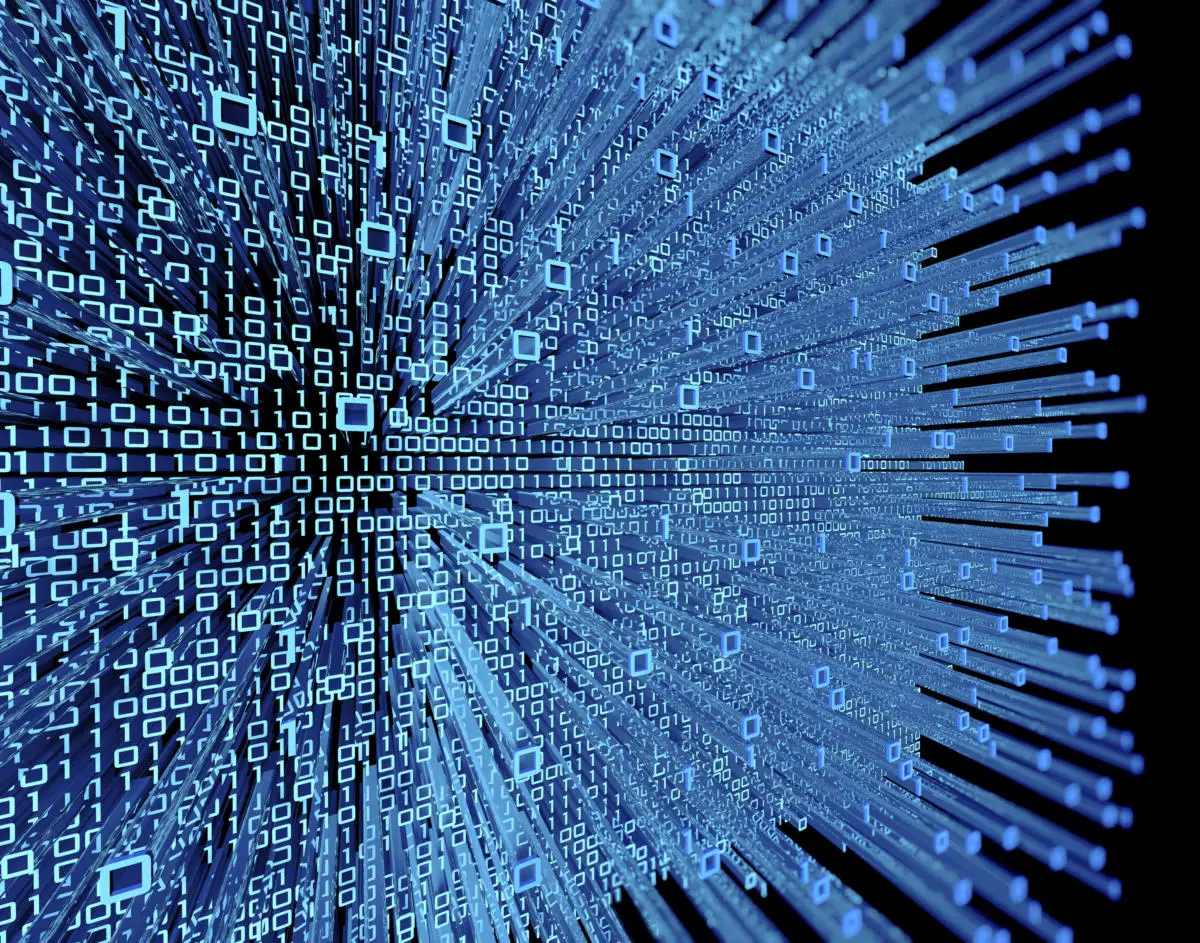
\includegraphics[scale=0.25]{img/page_de_garde.png} \\[1cm]
        \HRule \\[0.4cm]
        { \huge \bfseries LINMA2710 Scientific Computing \\[0.4cm] }
    
        \HRule \\[1.5cm]
        \textsc{\LARGE Issambre L'Hermite Dumont \\ Simon Desmidt}\\[1cm]
        \vfill
        \vspace{2cm}
        {\large Academic year 2024-2025 - Q2}
        \vspace{0.4cm}
         
        
\includegraphics[width=0.15\textwidth]{img/epl.png}
        
        UCLouvain\\
    
    \end{center}
    \end{sffamily}
\end{titlepage}

\setcounter{tocdepth}{1}
\tableofcontents
\chapter{Shared-Memory Multiprocessing}
\section{How memory works}
\subsection{Memory hierarchy} 
To store the data that it will use, the CPU uses memory. Memory is hierarchical like a pyramid. The higher it is, the faster it goes, but the less space there is.
\begin{figure}[H]
    \centering
    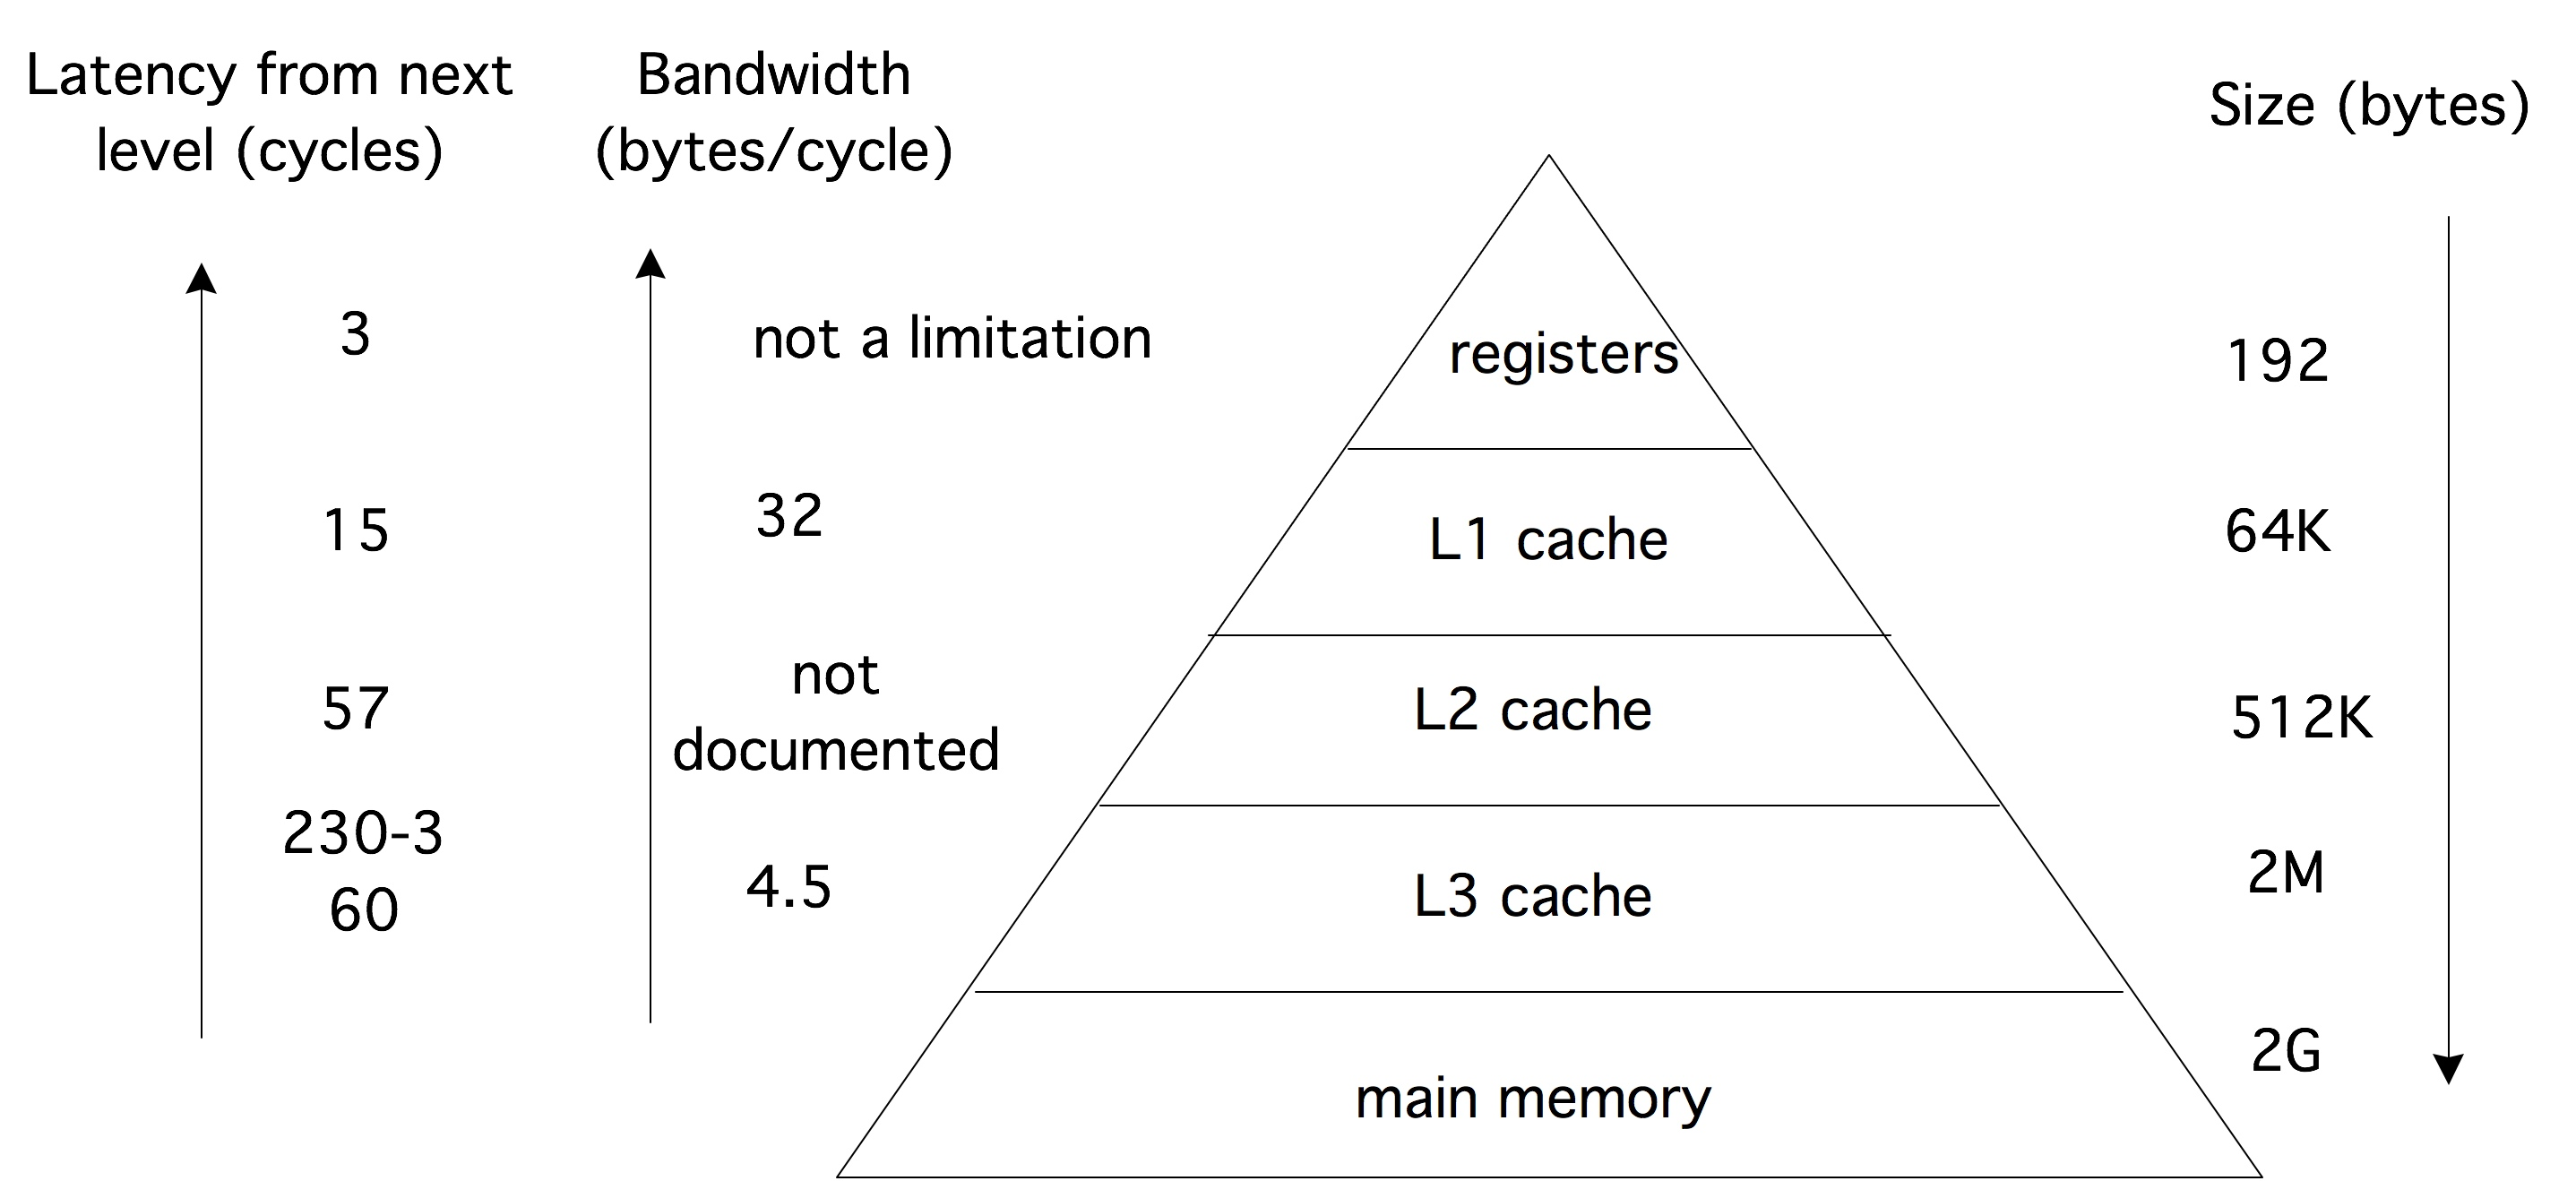
\includegraphics[scale=0.15]{img/memory_layout.jpeg}
    \caption{Memory hierarchy}
    \label{fig:memory_hierarchy}
\end{figure}
First we need to define a cycle\label{cycle_def}. It's an unit of time that is defined like this: $cycle = \frac{1}{\text{CPU freq}}$. For example, for the CPU \textit{AMD Ryzen 5 5600X}, the maximum frequency is $4.6 GHz$, so the cycle is $cycle = \frac{1}{4.6 GHz} \approx 0.217 ns$. The \textbf{bandwidth} is the number of bytes that can be transferred in one cycle. And the \textbf{latency} is the number of cycles required to access a level of memory. There's also the \textbf{latency} \label{def_latency} but for a number of bytes, its formula is $\alpha + \beta n$ where $\alpha$ is the level latency, $\beta$ is the inverse of the bandwidth and $n$ is the number of bytes.\\
\begin{tabularx}{\textwidth}{|c|X|X|X|X|X|}
	\hline
	Level & Level \newline Latency $[cycle]$  & Bandwidth $[bytes/cycle]$ & Size & What \newline is stored & Example \\
	\hline
	Register & $3$ & No limit & $\approx 192B$ & "Immediate" data for the CPU & Results of addition, memory address\\
	\hline
	Cache L1 & $15$ & $32-64$ & $\approx 64KB$ & Instructions and \newline "Immediate" data & Local \newline variable\\
	\hline
	Cache L2 & $57$ & $16-32$ & $\approx 512KB$ & Data used recently & Data struct, code part\\
	\hline
	Cache L3 & $230-360$ & $4-10$ & $\approx 64MB$ & Data shared between core& Global \newline variable\\
	\hline
	RAM & $300-500$ & $9-50GB/s$ & $\geq 4GB$ & Running programs & Running software, open \newline document\\
	\hline
	Disks & $\geq 10^5$ & Usually $\leq 3GB/s$ & $\geq 128GB$ & Persistent data & Document, OS, etc\\
	\hline
\end{tabularx}
\subsection{Caches lines and prefetching}\label{caches_lines}
A \textbf{cache line} is a small fixed-size contiguous block of memory, usually $64$ or $128$ bytes. It's not necessarily stored in the cache. We use them to organize the memory, because it is easier to deal with fixed size block. When the CPU need to access a memory location, it loads the entire cache line into the cache of the CPU.
If the wanted data is not in the cache, there will be a \textbf{cache miss}. After that the CPU will load the entire cache line into the cache.\\
The \textbf{prefetching} is the fact that the CPU will load the cache line that is next to the one that is needed. It's because of the spacial locality. Spacial locality is the reason why we use cache lines. For example, if we store an array of data, it may use some space greater than one cache line so for precaution, the CPU will load the next cache line too. And so we save time, by anticipating.\\
The data locality is important for at least the two following reasons:
\begin{itemize}
	\item \textbf{Temporal locality}: If a data is used frequently, we will keep it in the cache.
	\item \textbf{Spacial locality}: If a data is used, the data next to it could be useful too.
\end{itemize}
\newpage
\subsection{Arithmetic intensity}
The \textbf{arithmetic intensity} is a concept in performance analysis for memory-bound and compute-bound programs.
Let's consider a program that does $o$ arithmetic operations and $m$ memory operations, we define:
\begin{itemize}
	\item \textbf{Arithmetic intensity}: 
	\begin{equation} 
		a = \frac{o}{m}
	\end{equation}
	It helps find if the program is limited by a compute-bound or memory-bound.
	\item \textbf{Arithmetic time}: 
	\begin{equation} 
		t_{arith} = \frac{o}{\text{CPU freq}}
	\end{equation}
	It's the time needed to perform $o$ operations.
	\item \textbf{Memory transfer time}:
	\begin{equation} 
		t_{mem} = \frac{m}{\text{bandwidth}} = \frac{o}{a \times \text{bandwidth}}
	\end{equation}
	It's the time needed to do $m$ memory operations. 
\end{itemize}
The overall performance of a program is thus defined by the worst component of the PC, and so we get the \textbf{time per iteration}:
\begin{equation}
	\min \left( \frac{t_{arith}}{o},\frac{t_{mem}}{o} \right)
\end{equation}
With some algebra, we can find the \textbf{number of operations per second}:
\begin{equation}
	\max \left( \text{CPU freq}, a \times \text{bandwidth} \right)
\end{equation}
To resume:
\begin{itemize}
	\item If $a$ is low then the performance is memory-bounded $\Rightarrow$ \textbf{Need cache optimization}.
	\item If $a$ is high then the performance is compute-bounded $\Rightarrow$ \textbf{Need more CPU cores or vectorization}.
\end{itemize}
The arithmetic intensity can be represented with the \textbf{roofline model} which we'll talk about now.
\newpage
\subsection{The roofline model}
The two following graphs link the performances of a program with the arithmetic intensity. The "performances" means the number of operations per second and the "arithmetic intensity" is the number of operations per byte of memory transferred. The left graph is the case where we consider a perfect usage of the PC, and the right graph is the case where we consider a bad usage of the PC.  
\begin{figure}[H]
	\begin{subfigure}[b]{0.45\textwidth}
		\centering
		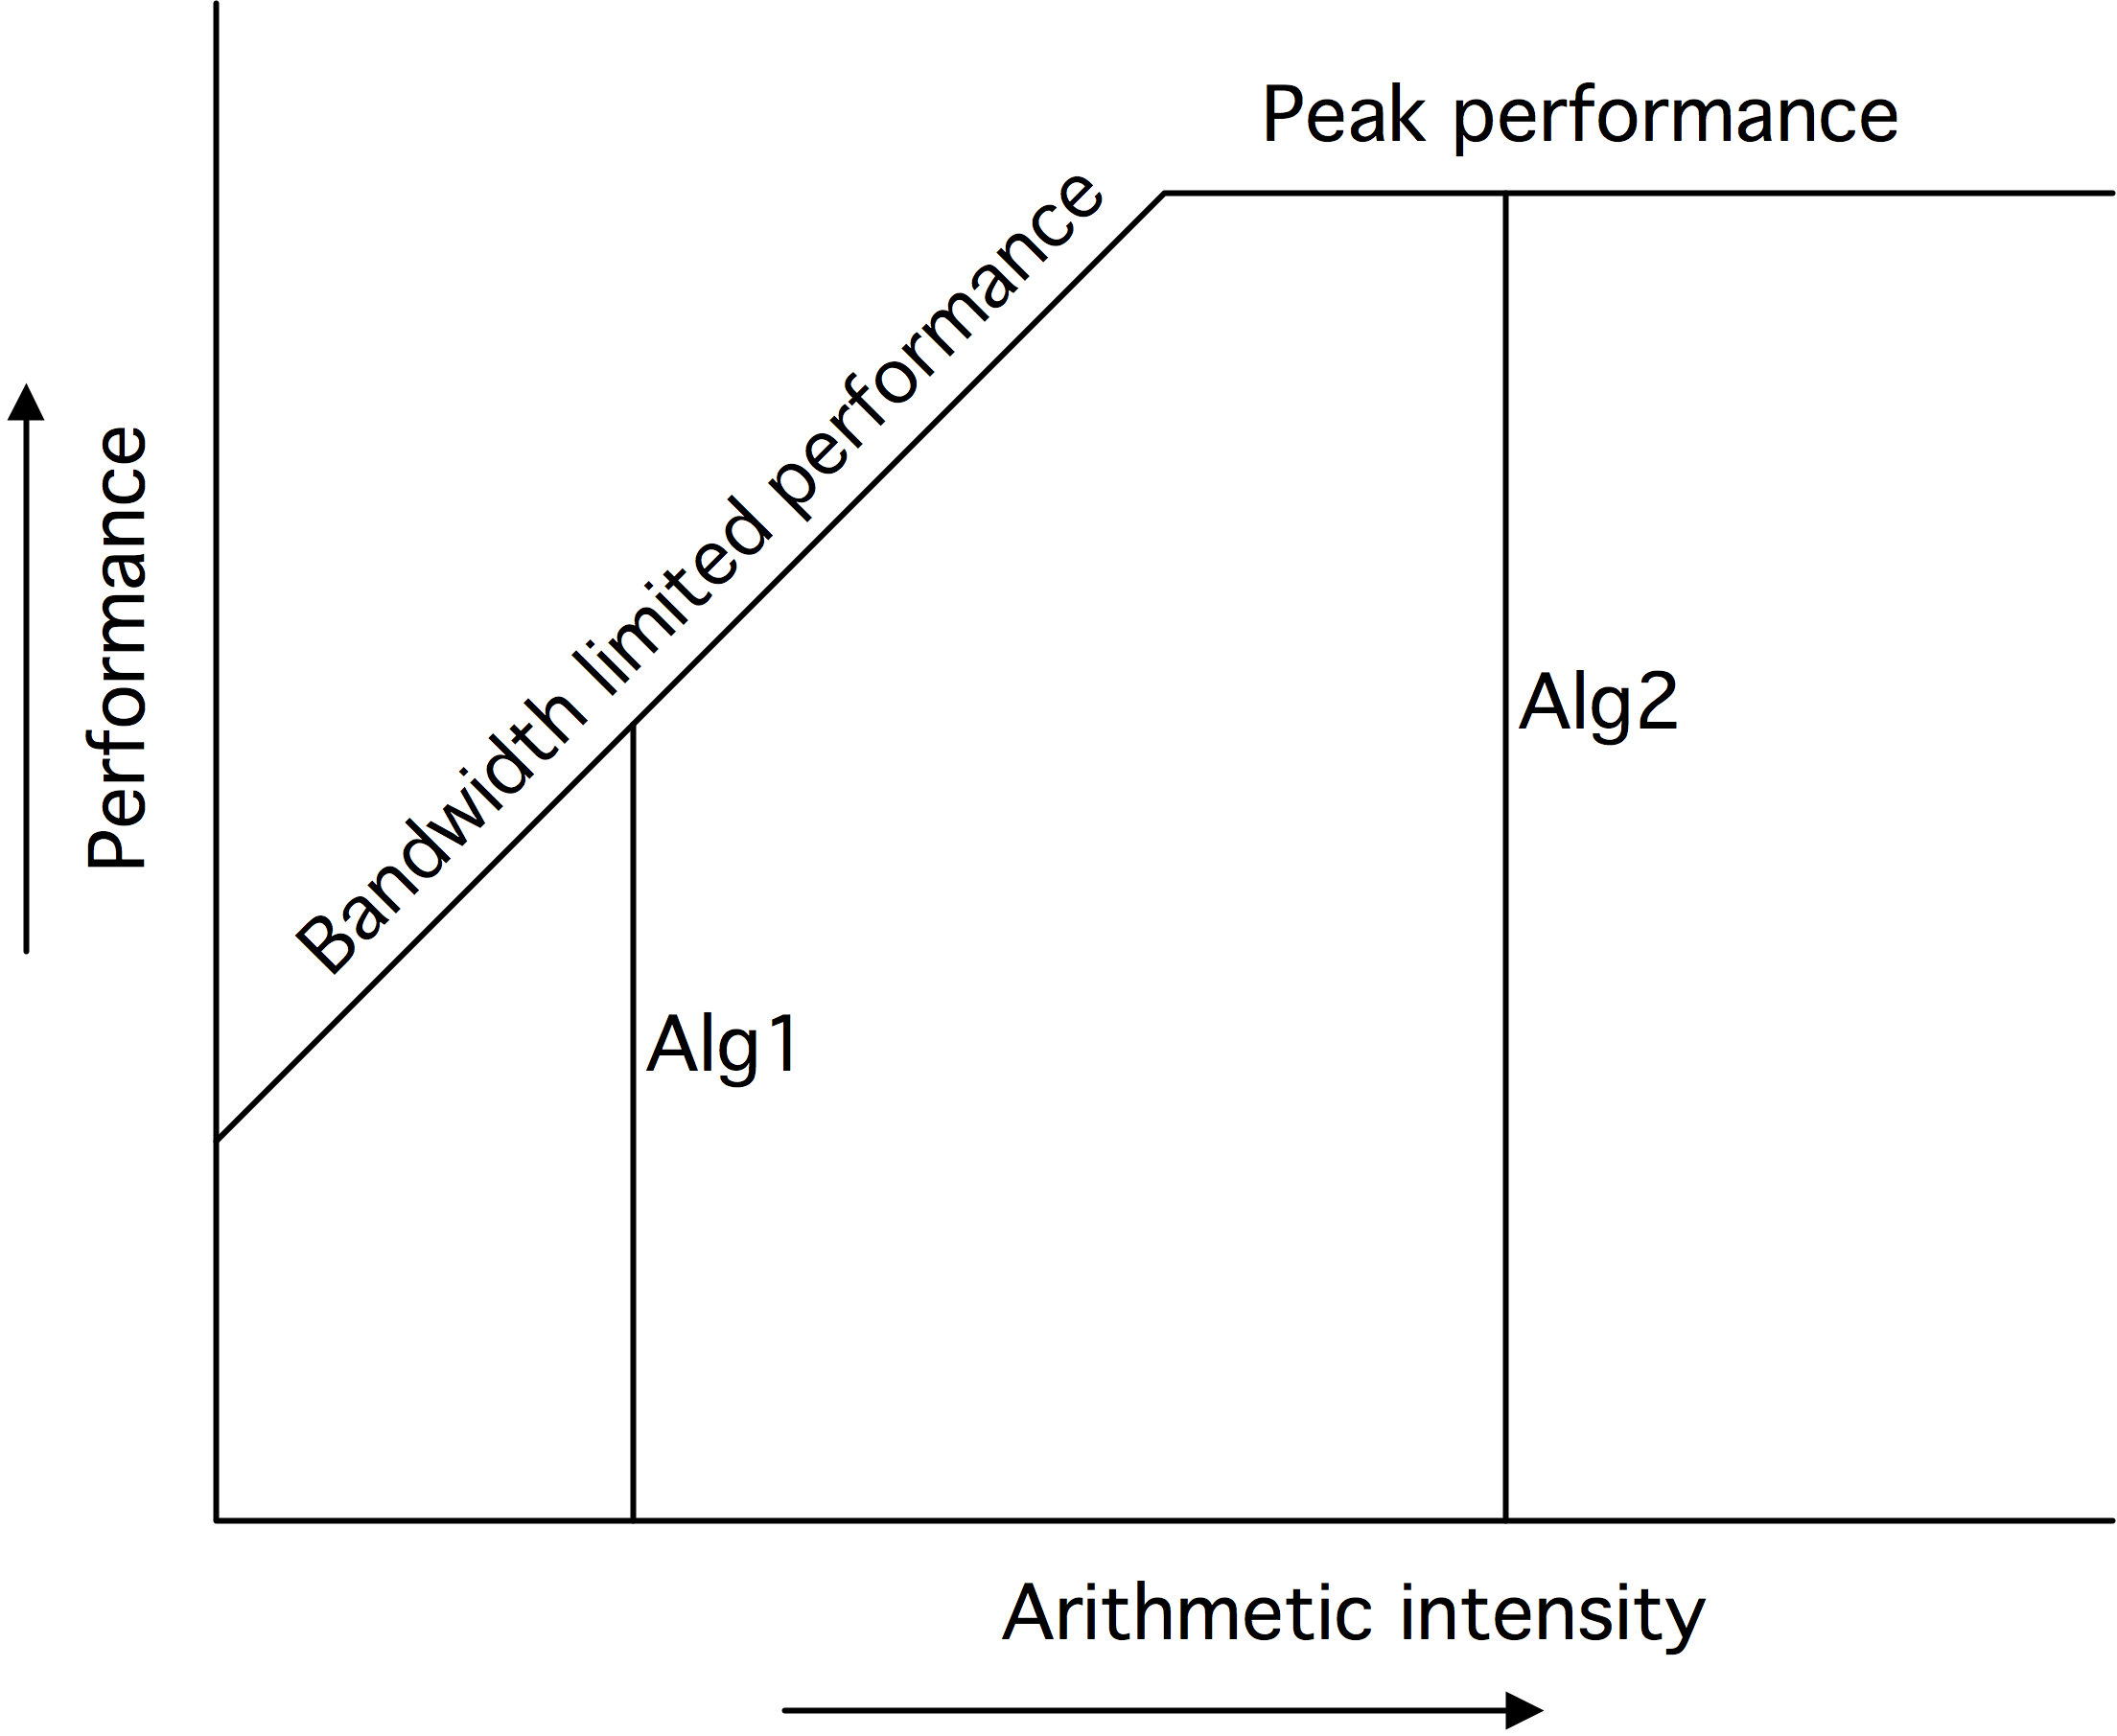
\includegraphics[scale=0.10]{img/roofline.jpeg}
		\caption{Roofline model}
		\label{fig:roofline}
	\end{subfigure}
	\begin{subfigure}[b]{0.45\textwidth}
		\centering
		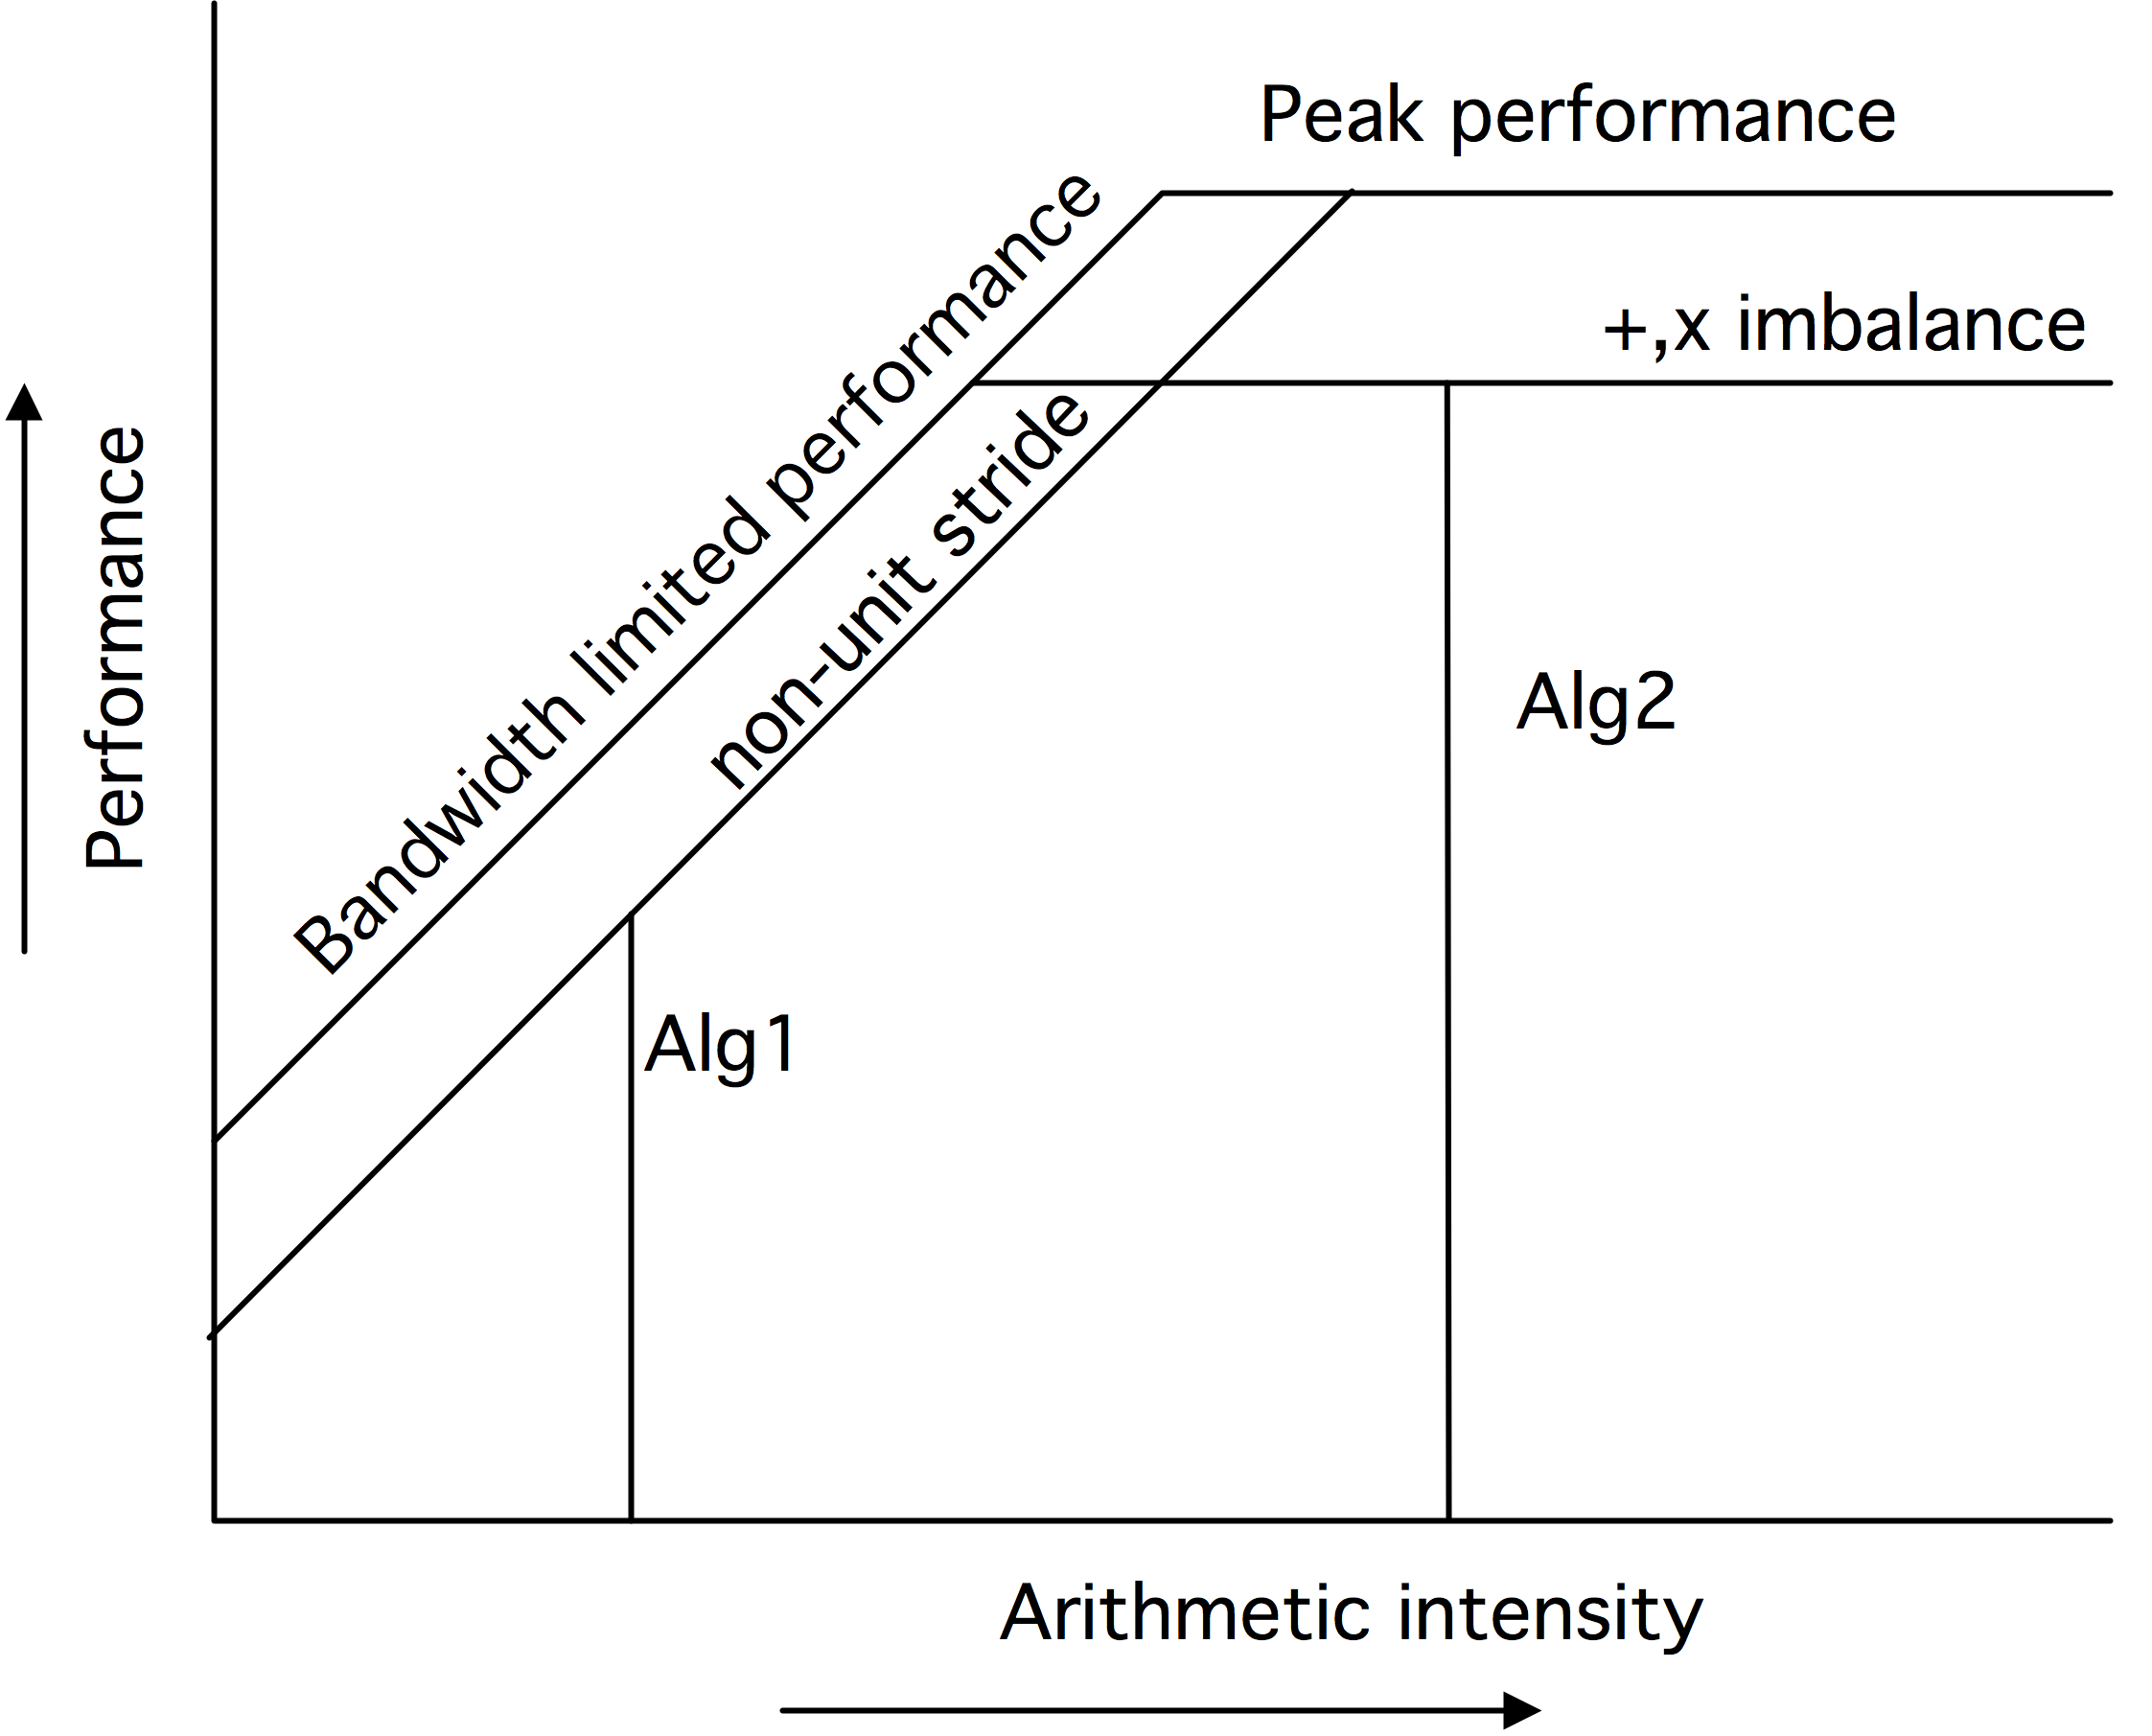
\includegraphics[scale=0.10]{img/roofline2.jpeg}
		\caption{Model with worse performances}
		\label{fig:roofline2}
	\end{subfigure}
\end{figure}
As we can clearly see, we have two limitations:
\begin{itemize}
	\item Bandwidth limit (slopped line)
	\item Computing limit (flat line)
\end{itemize}
These two limit lines are upper bounds for performances and are limited from above by the hardware (we can't do better than what our CPU can do), but they can be lower if the program is not optimized. For example the slopped line can be lower if we don't use the cache correctly. The flat line can be lower if we don't use the CPU correctly (e.g. not using SIMD).\\
\newpage
\subsection{Cache hierarchy for a multi-core CPU}
In the case where we have a multi-core CPU, the organization of the memory isn't always the same, it depends of the CPU architecture. For example, we can have a hierarchy like this:
\begin{figure}[H]
	\centering
	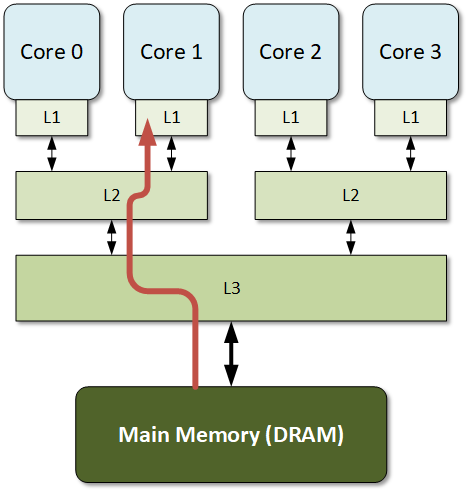
\includegraphics[scale=0.5]{img/multicore-cache.png}
	\caption{Cache hierarchy for a multi-core CPU}
	\label{fig:multi_core_cache}
\end{figure}
Here the L1 cache is private to each core, the L2 cache is shared between two cores and the L3 cache is shared between all cores, as well as the RAM. 
\section{Parallelism}
In this course, we use \textit{OpenMP} to parallelize our code instead of \textit{lpthread}. The advantages of \textit{OpenMP} are detailed in the chapter \textbf{useful tools} at the section \ref{OpenMP}.\\ 
Parallelism is a very useful tool to optimize the performances of a program. It allows to use multiple cores of the CPU to do multiple tasks at the same time. But sometimes it may arise some problems of performances or computational error.
\subsection{Computational error}
When using multi-threading, we may modify and use some variables at the same time which could cause computational error. So to avoid that we can either protect the variable (with some adapted tools) but this option is not very efficient because it takes some time to \textit{lock} and \textit{unlock} and to wait for the variable to be available. Or we can make each thread use its own version of the variable, this introduces the next problems.
\subsection{Race condition}
The race condition is a problem that occurs when two or more threads try to modify the same variable at the same time, here there are no computational error possible. For example if all the threads want to modify a variable a the same time, they will need to wait for the variable to be available, and it is a waste of time. The solution for that, as we said before is to make each thread use its own version of the variable. Let's say they need to compute the sum of an array. The solution is to make each thread compute the sum of a part of the array and then by "reduction" sum all the sums. We will see this in more detail in the next chapter.
\subsection{False sharing}
As we say before, in the section \ref{caches_lines} about cache lines, the CPU loads the entire cache line into the cache when it need to use some data that is on the cache line. So here is the problem, let's say that all of the partial sum of the array are stored in the same cache line, when a thread modify its partial sum, the entire cache line is loaded into the cache of the CPU, and so the other threads will have to wait for the cache line to be available. The solution is to make each thread use its own cache line. We can solve this by adding some padding (shift the data) to the data structure.
\section{Amdahl's law}
First let's define the \textbf{speedup} of a program, it represents the improvement of running time while using $p$ threads. It is defined by:
\begin{equation}
	S_p = \frac{T_1}{T_p}
\end{equation}
Where $T_1$ is the time needed to run the program with one thread and $T_p$ is the time needed to run the program with $p$ threads.\\
Then let's define the \textbf{efficiency} of a program, is mesures how well the parallelization is done. It is defined by:
\begin{equation}
	E_p = \frac{S_p}{p}
\end{equation}
Where $S_p$ is the speedup of the program with $p$ threads. We get 3 cases:
\begin{itemize}
	\item If $E_p = 1 \Rightarrow$ \textbf{Ideal case}, the parallelization is perfect.
	\item If $E_p < 1 \Rightarrow$ \textbf{Realistic case}, there's some inefficiency.
	\item If $E_p > 1 \Rightarrow$ \textbf{Unrealistic case}, would imply a super-linear speedup.
\end{itemize}
We can now define \textbf{Amdahl's law}, which explain the limitation of parallelization due to the presence of a sequential portion in a program. It is defined like this:
\begin{equation}
	T_p = F_sT_1 + \frac{(1 - F_s)T_1}{p}
\end{equation}
$F_s$ is the percentage of the program that is sequential (impossible to parallelize). With that we can redefine the \textbf{speedup} and the \textbf{efficiency} of a program:
\begin{equation}
	S_p = \frac{T_1}{F_sT_1 + \frac{(1 - F_s)T_1}{p}} = \frac{1}{F_s + \frac{1 - F_s}{p}} \Rightarrow \lim_{p \to \infty} S_p = \frac{1}{F_s}
\end{equation}
And
\begin{equation}
	E_p = \frac{S_p}{p} = \frac{1}{pF_s + 1 - F_s} = \frac{1}{F_s(p - 1) + 1}
\end{equation}
\begin{figure}[H]
	\centering
	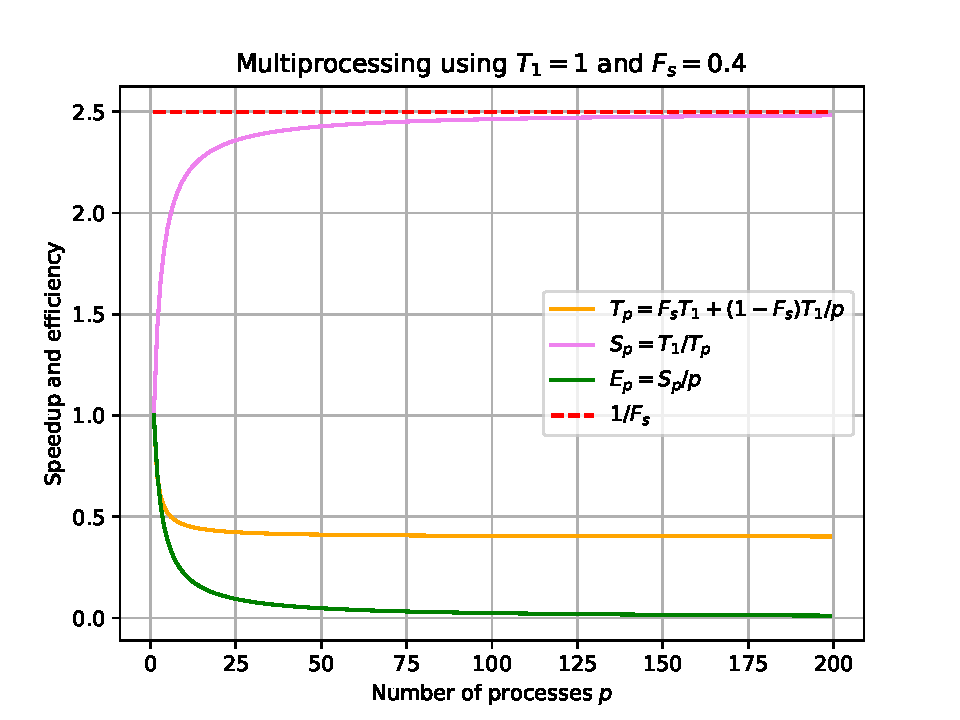
\includegraphics[width=0.8\linewidth]{img/amdahl.pdf}
	\caption{Amdahl's law}
	\label{fig:amdahl}
\end{figure}
\subsection{Application of Amdahl's law to parallel sum}
Let's consider the sum of an array, we want to parallelize it. The time without parallelization is $n$ and with parallelization is $\frac{n}{p} + \log_2(p)$, the log term is the time needed to sum all the partial sums. So the speedup is:
\begin{equation}
	S_p = \frac{n}{\frac{n}{p} + \log_2(p)} = \frac{1}{\frac{1}{p} + \frac{\log_2(p)}{n}}
\end{equation}
And the efficiency is:
\begin{equation}
	E_p = \frac{S_p}{p} = \frac{1}{1 + \frac{p}{n}\log_2(p)}
\end{equation}
We clearly see that if we use more than $n$ processes the efficiency will decrease. Because if $p \geq n$ then we have $T_p = \log_2(n)$ and $\lim_{p \to \infty} S_p = \frac{1}{\log_2(n)}$ and $F_s = \log_2(n)$
\chapter{Single Instruction Multiple Data (SIMD)}
\textcolor{red}{Maybe to improve}\\
SIMD (Single Instruction Multiple Data) is a parallel computing architecture used to process multiple data points simultaneously with a single instruction.\\
The idea of SIMD is that instead of executing the same instruction separately for each data element, SIMD processes multiple elements in parallel within a single CPU cycle. To simplify SIMD takes advantages of \textbf{vectorization}, to optimize the performances of the program. It uses register to store the vector on which it does the computing.\\
Let's do a little example, consider the following code:
\begin{lstlisting}[style=CppStyle]
	int a[] = {...};
	int b[] = {...};
	int c[size];
	for(int i = 0; i < size; i++){
		c[i] = a[i] + b[i];
	}
\end{lstlisting}
Here we use \texttt{int} which is $32$ bytes so if we use SIMD with AVX2 registers, we can store $(512/32 =) 16$ integers in a register. And so SIMD with that type of registers will automatically translate the previous code to:
\begin{lstlisting}[style=CppStyle]
	int a[] = {...};
	int b[] = {...};
	int c[size];
	for(int i = 0; i < size; i+=16){
    __m512_add_epi16(c+i, a+i, b+i);
	}
\end{lstlisting}
We can write the code with the intrinsics (\code{\_\_m512\_add\_epi16}) but it's not necessary. The compiler will do it for you.\\
To use SIMD, you need to give to your compiler some flags, for example:
\begin{itemize}
	\item \code{-O2} or \code{-O3} for optimization
	\item \code{-mavx} for AVX
	\item \code{-mavx2} for AVX2
	\item \code{-mavx512} for AVX512
\end{itemize}
\textcolor{red}{TODO: explain AVX}\\
\chapter{Distributed Computing with MPI}
\section{Single Program Multiple Data (SPMD)}
Single Program Multiple Data means that we make multiple processes execute the same program but operate on different data. It's a kind of parallel computing that we call distributed computing.
\subsection{Message Passing Interface (MPI)}
MPI is a standardized and portable message-passing system used to enable parallel computing across multiple nodes.
Here are some key steps with MPI:
\begin{itemize}
	\item Initialization: \code{MPI\_Init(\&argc, \&argv);}, initialize MPI and the processes.
	\item Getting the number of processes: \code{MPI\_Comm\_size(MPI\_COMM\_WORLD, \&nprocs);}, determines how many processes are running (\code{nprocs} is the same for all processes.)
	\item Getting the rank of the process: \code{MPI\_Comm\_rank(MPI\_COMM\_WORLD, \&procid);} Give a unique ID (rank) to each process, which allows them to perform different tasks despite running the same program.
	\item Finalizing MPI:  \code{MPI\_Finalize();}, finalize MPI and free the ressources.
\end{itemize}
\newpage
\section{Collectives}
Let's consider a system that can support $4$ processes for the explicit examples (tables). And for the bounds consider as usual $p$ process and the variables defined for the latency \ref{def_latency} ($\alpha,\beta,n$) and an arithmetic intensity parameter ($\gamma$). Here is some illustration of how collectives work:
\begin{figure}[H]
	\centering
	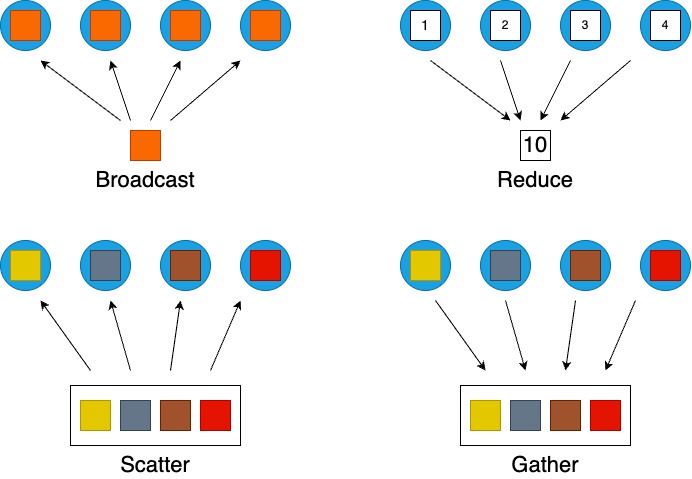
\includegraphics[scale=0.5]{img/collectives.jpeg}
	\caption{Collectives}
	\label{fig:collectives}
\end{figure}

\textcolor{red}{TODO: give the function for each and the args}
\subsection{Broadcast}
\textbf{Broadcast} makes a process gives a variable to the other processes.\\
\begin{center}
	\begin{tabular}{ccccc|c|ccccc}
		Before &&&&& $\Longrightarrow$ &After&&&&\\
		\hline
		procid & 0 & 1 & 2 & 3 & & procid & 0 & 1 & 2 & 3\\
		\hline
		& $x$ &&&&& & $x$ & $x$ & $x$ & $x$\\
		\hline
	\end{tabular}
\end{center}
Using \textit{spanning tree algorithm}, we can \textbf{broadcast} in $\log_2(p)(\alpha + \beta n)$.
\subsection{Gather}
\textbf{Gather} makes a process gather the variables of the other processes.\\
\begin{center}
	\begin{tabular}{ccccc|c|ccccc}
		Before &&&&& $\Longrightarrow$ &After&&&&\\
		\hline
		procid & 0 & 1 & 2 & 3 & & procid & 0 & 1 & 2 & 3\\
		\hline
		& $x_0$ &&&&& & $x_0$ &&&\\
		&& $x_1$ &&&& & $x_1$ &&&\\
		&&& $x_2$ &&& & $x_2$ &&&\\
		&&&& $x_3$ && & $x_3$ &&&\\
		\hline
	\end{tabular}
\end{center}
Using \textit{spanning tree algorithm}, we \textbf{gather} in $\log_2(p)\alpha + \beta n$.
\subsection{Reduce}
\textbf{Reduce} sums up all the values of the variables on the differents processes and store the sum on one process.\\
\begin{center}
	\begin{tabular}{ccccc|c|ccccc}
		Before &&&&& $\Longrightarrow$ &After&&&&\\
		\hline
		procid & 0 & 1 & 2 & 3 & & procid & 0 & 1 & 2 & 3\\
		\hline
		& $x_0$ & $x_1$ & $x_2$ & $x_3$ && & $\displaystyle \sum_{i=0}^{3} x_i$ &&&\\
		\hline
	\end{tabular}
\end{center}
Using \textit{spanning tree algorithm}, we can \textbf{reduce} in $\log_2(p)(\alpha + \beta n) + \log_2(p) \gamma n$. To simplify we have: $\log_2(p)(\alpha + (\beta + \gamma) n)$.
\subsection{All gather}
\textbf{All gather} is a sort of combination of \textbf{gather} and \textbf{broadcast}. It gathers all the variables of the processes and broadcast them to all the processes but more efficiently.\\
\begin{center}
	\begin{tabular}{ccccc|c|ccccc}
		Before &&&&& $\Longrightarrow$ &After&&&&\\
		\hline
		procid & 0 & 1 & 2 & 3 & & procid & 0 & 1 & 2 & 3\\
		\hline
		& $x_0$ &&&&& & $x_0$ & $x_0$ & $x_0$ & $x_0$\\
		&& $x_1$ &&&& & $x_1$ & $x_1$ & $x_1$ & $x_1$\\
		&&& $x_2$ &&& & $x_2$ & $x_2$ & $x_2$ & $x_2$\\
		&&&& $x_3$ && & $x_3$ & $x_3$ & $x_3$ & $x_3$\\
		\hline
	\end{tabular}
\end{center}
Using \textit{spanning tree algorithm}, we can \textbf{all gather} in $\log_2(p)\alpha + \beta n$.
\subsection{Reduce scatter}
\textbf{Reduce scatter} is a sort of combination of \textbf{reduce} and \textbf{scatter}. It reduces the variables of the processes and scatter them to all the processes, but more efficiently.\\
\begin{center}
	\begin{tabular}{ccccc|c|ccccc}
		Before &&&&& $\Longrightarrow$ &After&&&&\\
		\hline
		procid & 0 & 1 & 2 & 3 & & procid & 0 & 1 & 2 & 3\\
		\hline
		& $x_{0,0}$ & $x_{0,1}$ & $x_{0,2}$ & $x_{0,3}$ &&& $\displaystyle \sum_{j=0}^{3} x_{0,j}$ &&&\\
		& $x_{1,0}$ & $x_{1,1}$ & $x_{1,2}$ & $x_{1,3}$ &&&& $\displaystyle \sum_{j=0}^{3} x_{1,j}$ &&\\
		& $x_{2,0}$ & $x_{2,1}$ & $x_{2,2}$ & $x_{2,3}$ &&&&& $\displaystyle \sum_{j=0}^{3} x_{2,j}$ &\\
		& $x_{3,0}$ & $x_{3,1}$ & $x_{3,2}$ & $x_{3,3}$ &&&&&& $\displaystyle \sum_{j=0}^{3} x_{3,j}$ \\
		\hline
	\end{tabular}
\end{center}
Using \textit{spanning tree algorithm}, we can \textbf{reduce scatter} in $\log_2(p)\alpha + (\beta + \gamma) n$
\subsection{All reduce}
\textbf{All reduce} is a sort of combination of \textbf{reduce} and \textbf{broadcast}.\\
\begin{center}
	\begin{tabular}{ccccc|c|ccccc}
		Before &&&&& $\Longrightarrow$ &After&&&&\\
		\hline
		procid & 0 & 1 & 2 & 3 & & procid & 0 & 1 & 2 & 3\\
		\hline
		& $x_0$ & $x_1$ & $x_2$ & $x_3$ && & $\displaystyle \sum_{i=0}^{3} x_i$ & $\displaystyle \sum_{i=0}^{3} x_i$ & $\displaystyle \sum_{i=0}^{3} x_i$ & $\displaystyle \sum_{i=0}^{3} x_i$\\
		\hline
	\end{tabular}
\end{center}
We explained above that we can do a combination of \textbf{reduce} and \textbf{broadcast}, but we can \textbf{all reduce} more efficiently doing \textbf{reduce scatter} then \textbf{all gather}, and we can do it in $\log_2(p)\alpha + \beta n$.
\section{Point-to-point communication}
\begin{figure}[H]
	\centering
	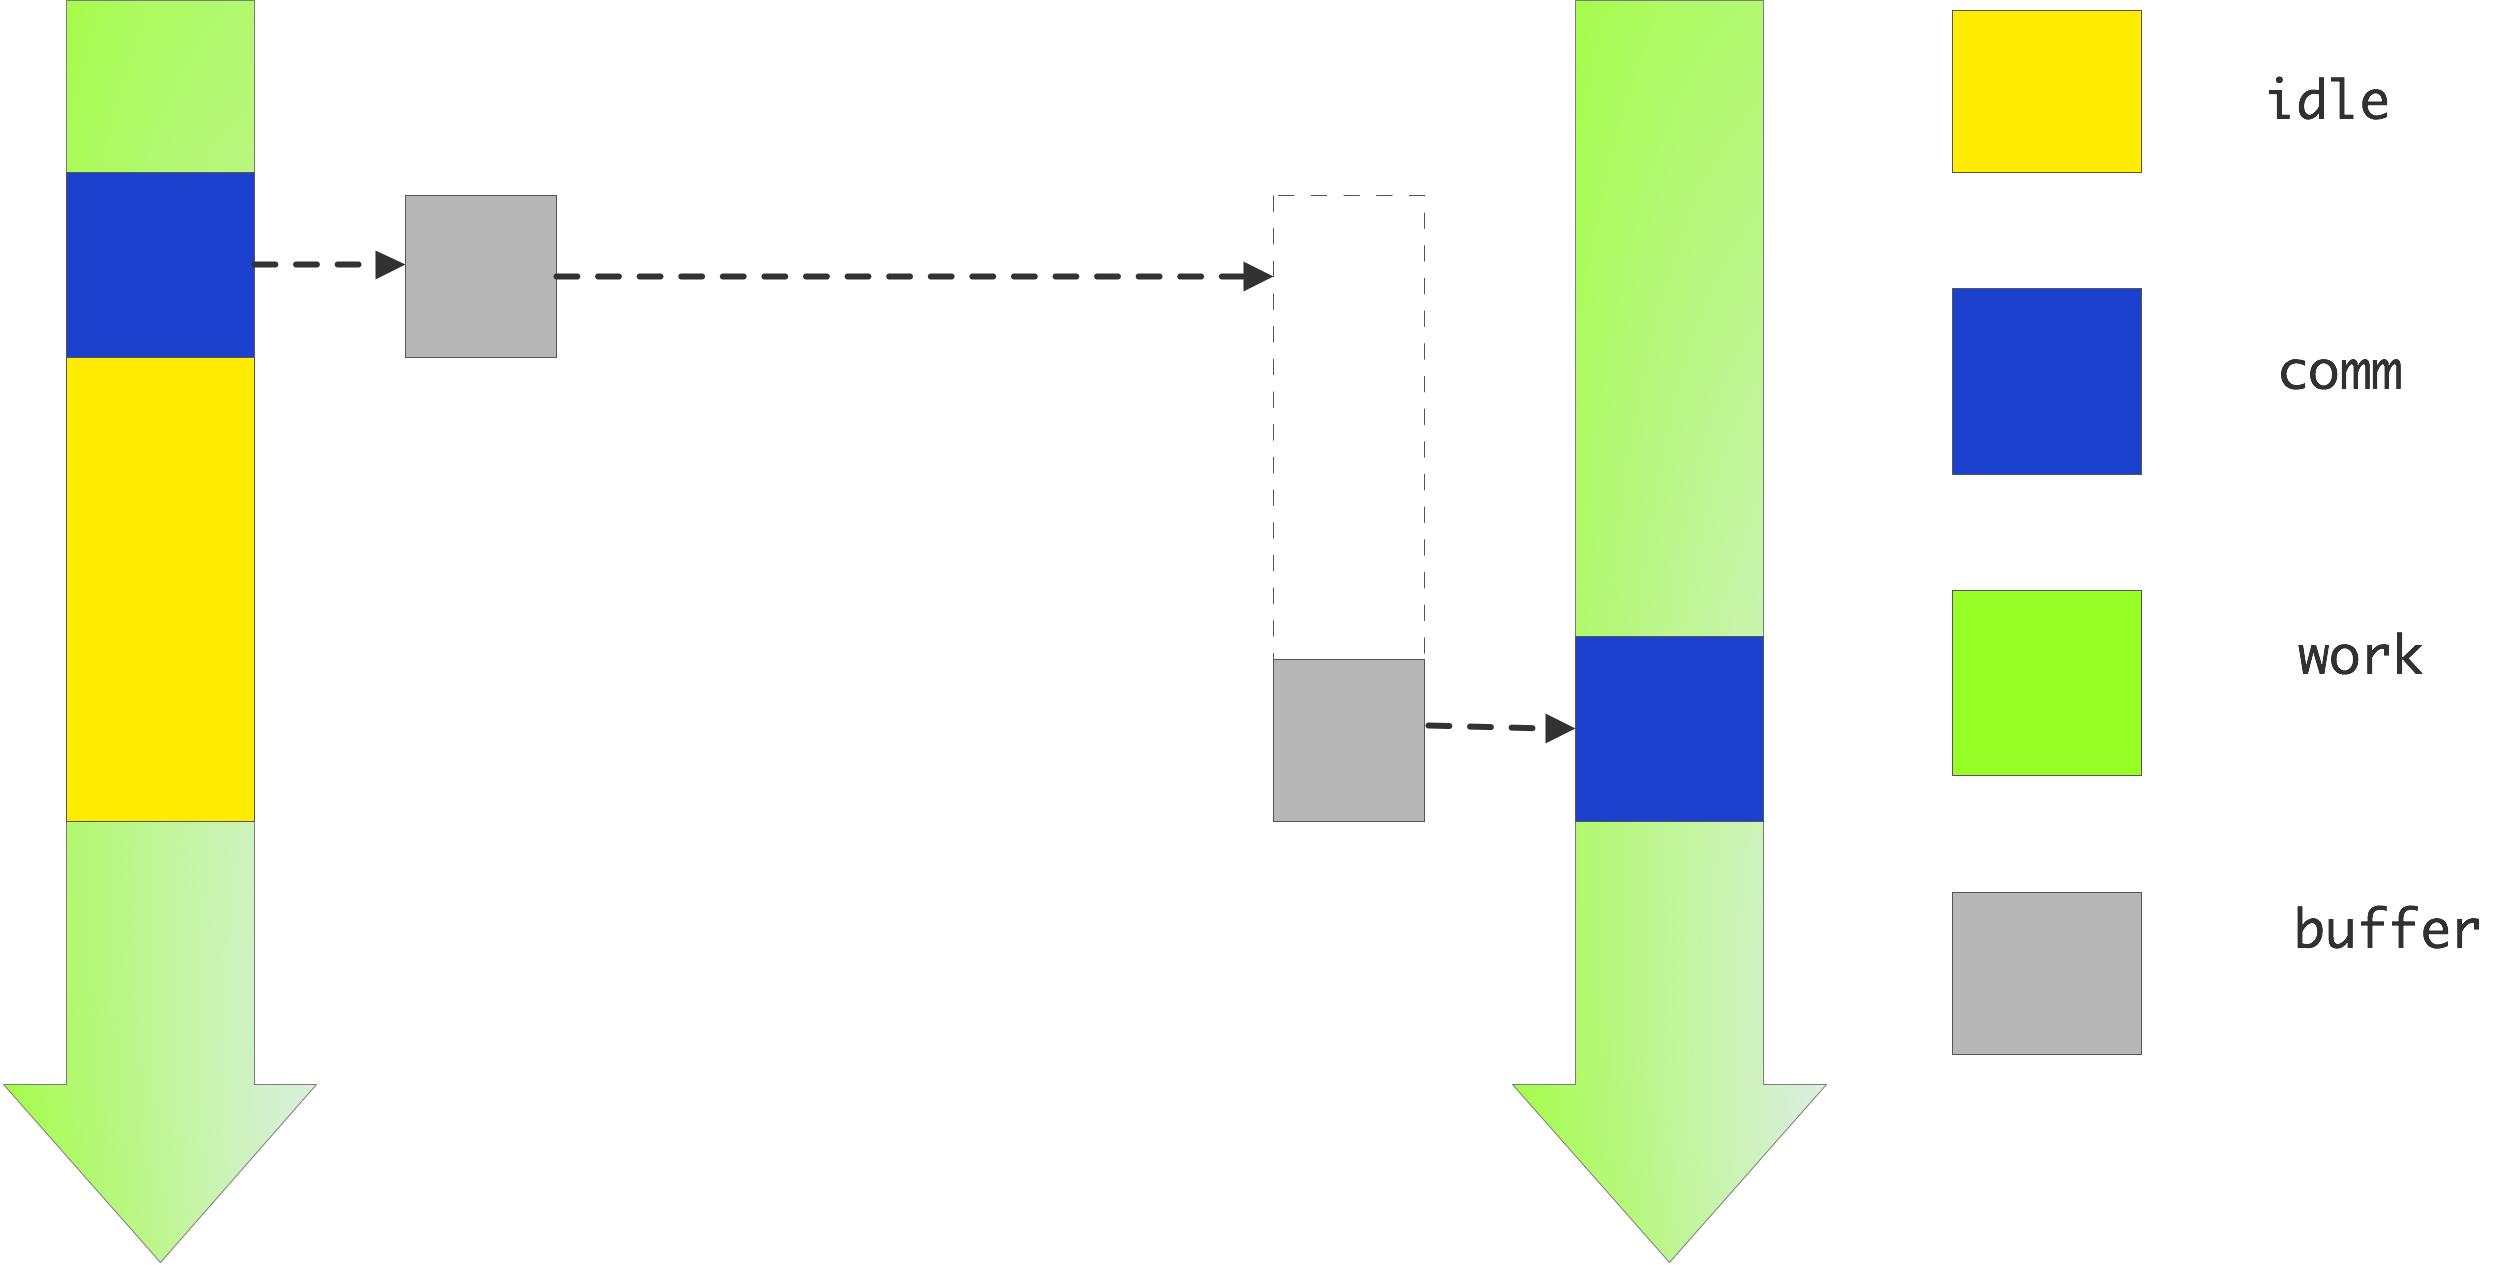
\includegraphics[width=0.8\linewidth]{img/com2.png}
	\caption{Point-to-point blocking communication}
	\label{fig:Com_block}
\end{figure}
This figure shows the problem of point-to-point blocking communication in MPI. As we can see, the left process is waiting for the right process to send the data, and thus is idling and wasting time. It does that because the sender cannot continue until the message is completely transferred. And in the case of a too big message that can't be stored in the buffer then the sender must wait for the receiver.\\
There is two ways to solve this problem:
\begin{itemize}
	\item \textbf{Rendezvous protocol}: It works like an handshake process, so we have:
	\begin{itemize}
		\item The sender sends a header to notify the receiver that he will send data.
		\item The receiver replies with a "ready-to-send" signal.
		\item The sender sends the actual data.
	\end{itemize}
	\item \textbf{Eager protocol}: The message is quickly buffered in the sender's buffer to allow \code{MPI\_Send()} to finish "eagerly" and when the receiver is ready, it can receive the message. The sender doesn't wait for the receiver to be ready. It's useful when the message is small and thus fit in the buffer.\\
\end{itemize}
The eager protocol can be represented like this:
\begin{figure}[H]
	\centering
	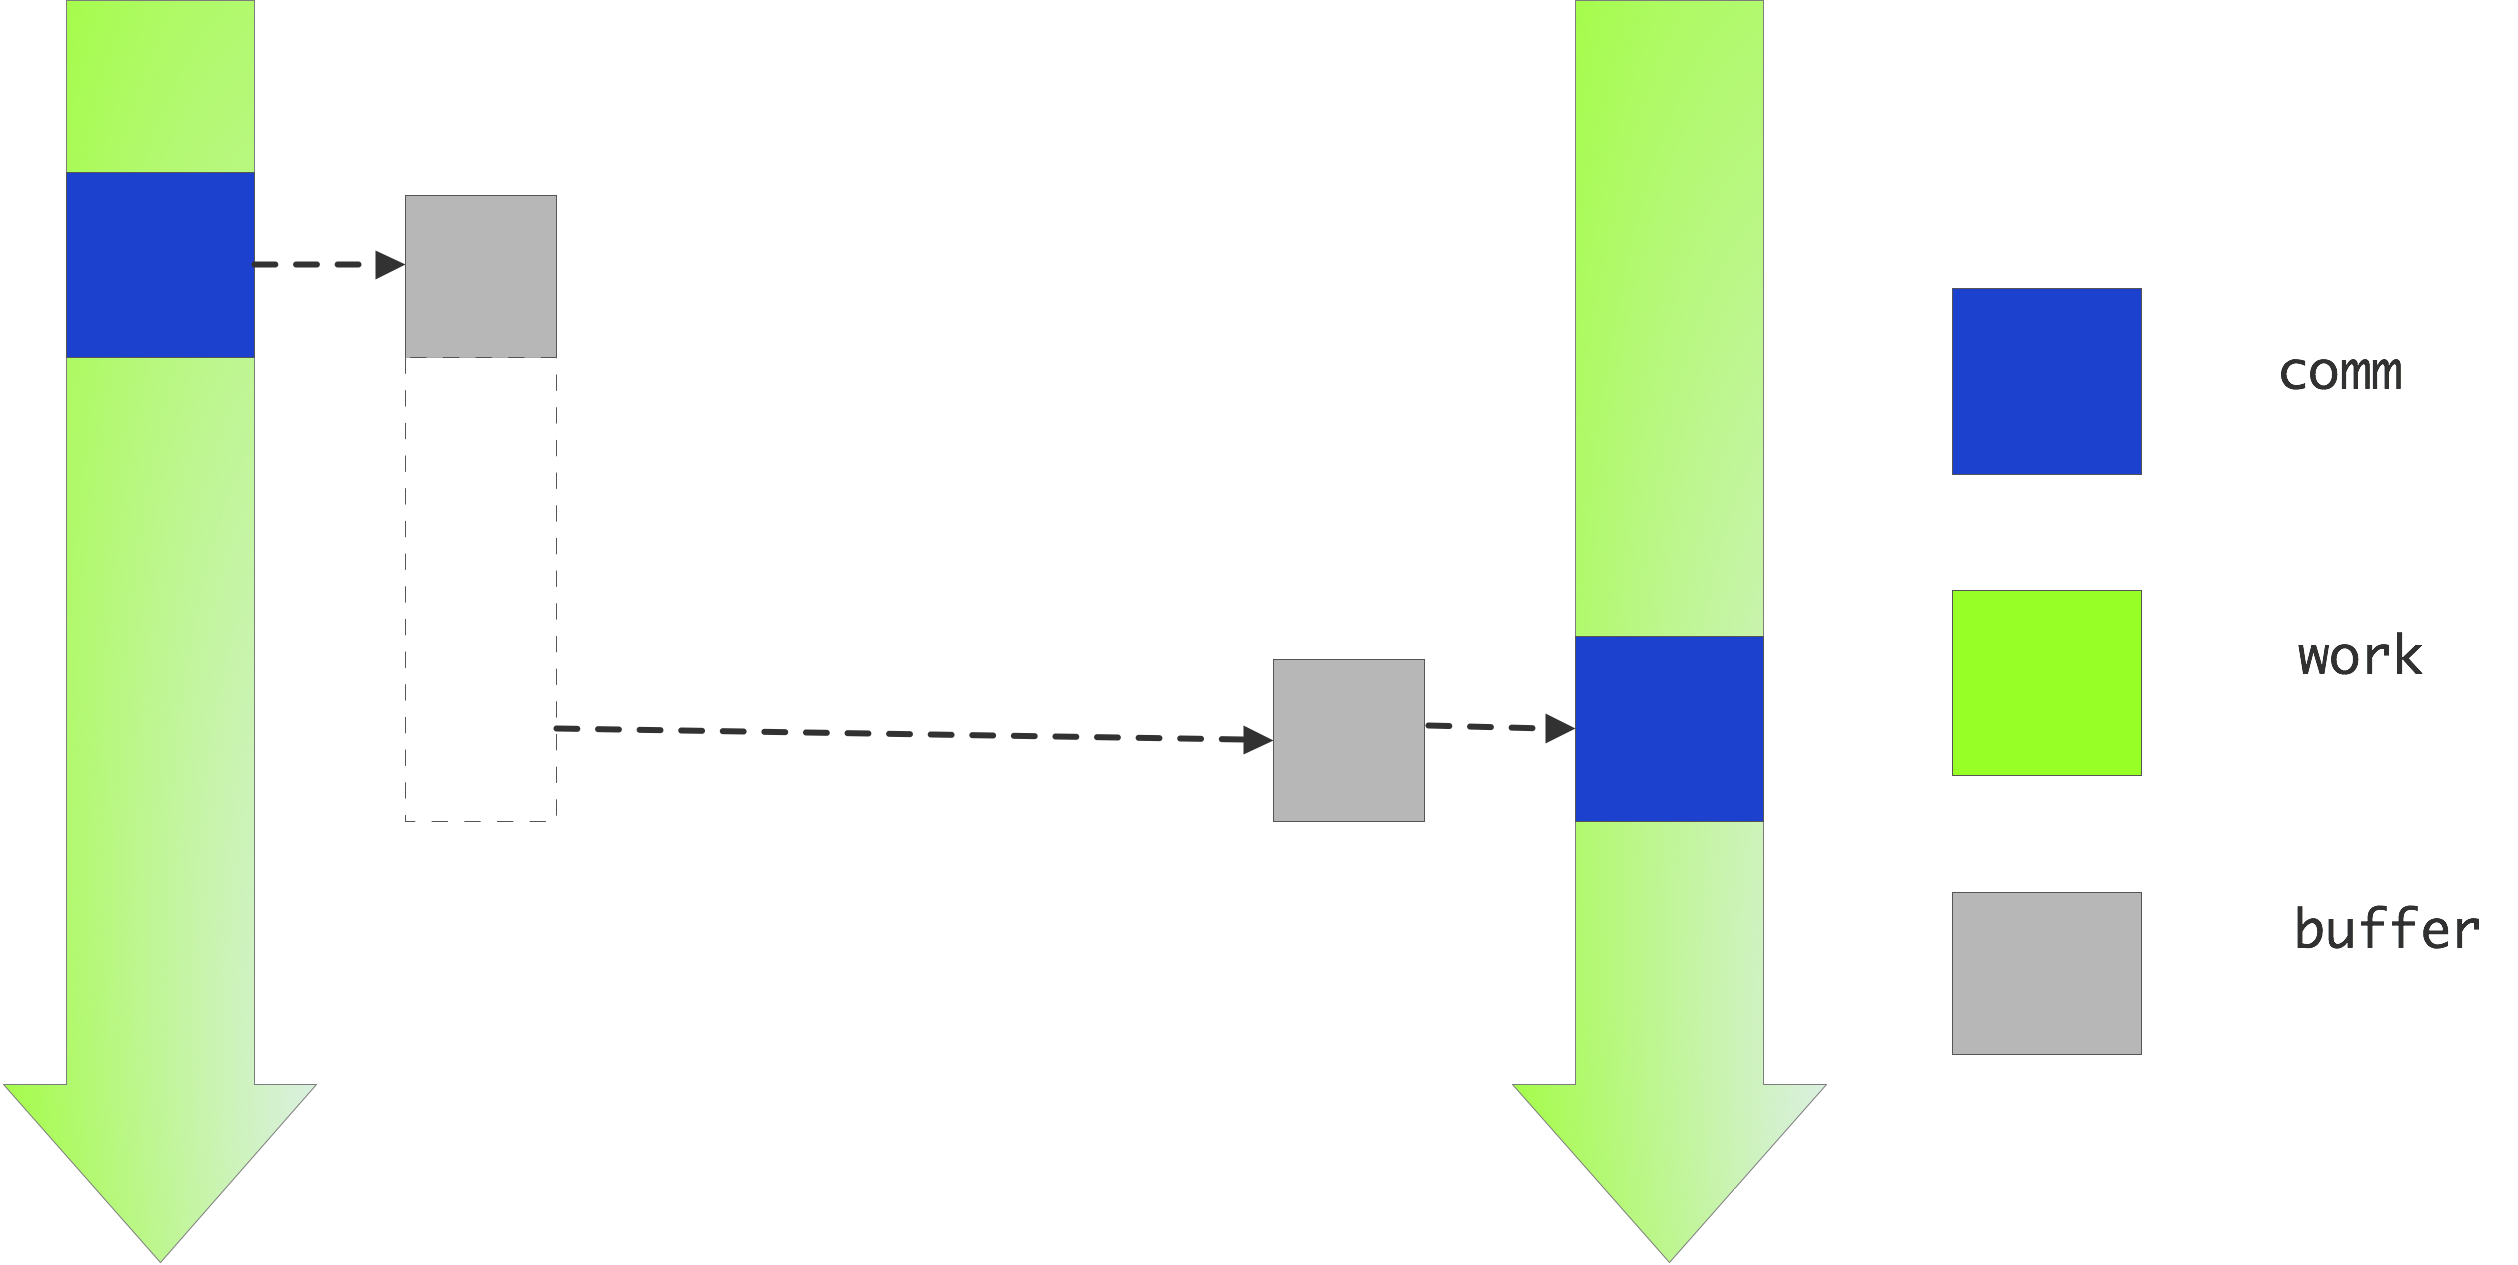
\includegraphics[width=0.8\linewidth]{img/eager.jpeg}
	\caption{Eager protocol}
	\label{fig:eager}
\end{figure}
\chapter{Scientific computing on GPU}
\section{What is a GPU?}
\subsection{GPU vs CPU}
A \textbf{GPU} (Graphics Processing Unit) is simply a CPU but specialized for parallel computing and is commonly used for matrix computations. In order to understand why let's do a little comparison between CPU and GPU:
\begin{center}
	\begin{tabular}{|c|c|c|}
		\hline
		& CPU & GPU \\
		\hline
		Purpose & brain of the PC & graphic rendering \\
		\hline
		Number of cores/threads & a few $2-32$ & thousands \\
		\hline
		Processing & serial work & parallel work \\
		\hline
		Memory (global) & RAM ($8-64< \: GB$) & VRAM ($4-24< \: GB$) \\
		\hline
		Memory (local) & cache L1, L2, L3 (cf \ref{fig:memory_hierarchy}) & $32-128 KB$ per block \\
		\hline
		Frequency & high ($3-5 GHz$) & low ($1-2 GHz$) \\
		\hline
		Flexibility & versatile & specialized \\
		\hline
	\end{tabular}
\end{center}
So to summarize, the CPU is a group of a few powerful worker that do different work each while the GPU have an army of workers that do the same simple task in parallel to contribute to a greater goal.\\
GPU are used commonly for graphics rendering, but it's not the only thing that they can do, we can use them for any kind of parallel computing. For example: machine learning, deep learning, simulations, etc. To do that we can run code using different "translation platforms" like \textbf{CUDA} (NVIDIA only), \textbf{ROCm} (AMD only) or open source alternative like \textbf{OpenCL}.\\
\newpage
\subsection{Hierarchy}
The hierarchy is pretty simple, we have the host that send the jobs to the rest of the CPU and GPU. After that, we have the computing devices. All of the cores of the CPU are managed as one, and each GPU is an independant computing device. After that, we have the computing units. Typically, for a CPU each core is a computing unit, and for a GPU each computing unit is composed a block of processors that can run multiples threads at the same time. And at the lowest level is the processing elements, it is an ALU (Arithmetic Logic Unit), to simplify it's a single thread that does basic operations.\\
\begin{figure}[H]
	\centering
	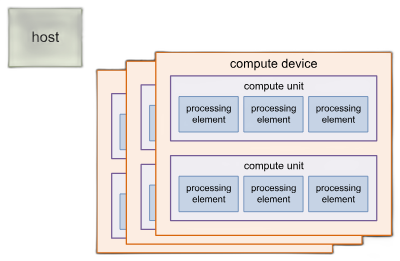
\includegraphics[width=0.8\linewidth]{img/hierarchy.png}
	\caption{Hierarchy}
	\label{fig:Hierarchy}
\end{figure}
And we can get informations from all of those levels by the following functions:
\begin{center}
	\begin{tabular}{|c|c|c|}
		\hline
		compute device & compute unit & processing element \\
		\hline
		get\_global\_id & get\_group\_id & get\_local\_id \\
		\hline
		get\_global\_size & get\_num\_groups & get\_local\_size \\
		\hline
	\end{tabular}
\end{center}
\newpage
\subsection{Memory hierarchy}
The memory hierarchy follows the same principle as the hierarchy. The host has its own memory (RAM). The global memory is the memory of the GPU, it is shared between all the threads of the GPU but is "slow" (VRAM). The local memory is shared between all the threads of a computing unit, and is faster than the global memory. And finaly the private memory is the memory of a thread, it is the fastest memory. The size of the memory is decreasing as its locality increases.\\
\begin{figure}[H]
	\centering
	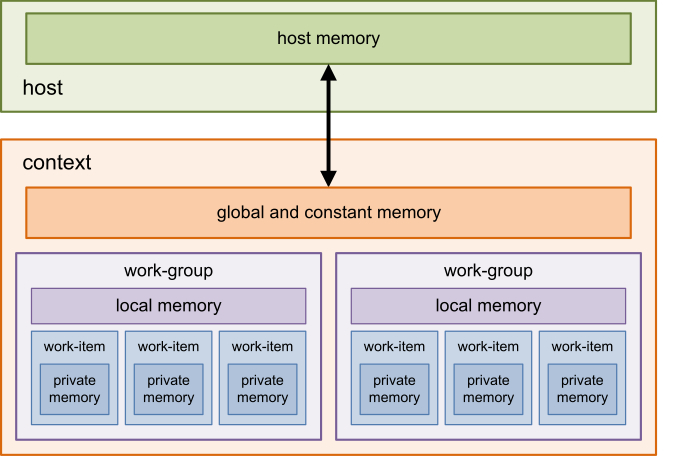
\includegraphics[width=0.8\linewidth]{img/mem_GPU.png}
	\caption{Memory hierarchy}
	\label{fig:mem_GPU}
\end{figure}
\chapter{Power consumption of computing}
\section{Power consumption of the components}
First we need to define the Thermal Design Power (TDP), it is the maximum amount of heat (in Watts) that a component is designed to dissipate. It is a useful measure to estimate the power consumption but also to design the cooling system.\\
\subsection{CPU}
The power of a CPU is approximately proportional to its utilisation until below $10\%$, so we can compute it like this:
\begin{equation}
	Power = TDP \times \max(0.1, \text{load})
\end{equation}
For example, for the CPU \textit{AMD Ryzen 5 5600X}, the TDP is $65W$, so we have this power curve:
\begin{figure}[H]
	\centering
	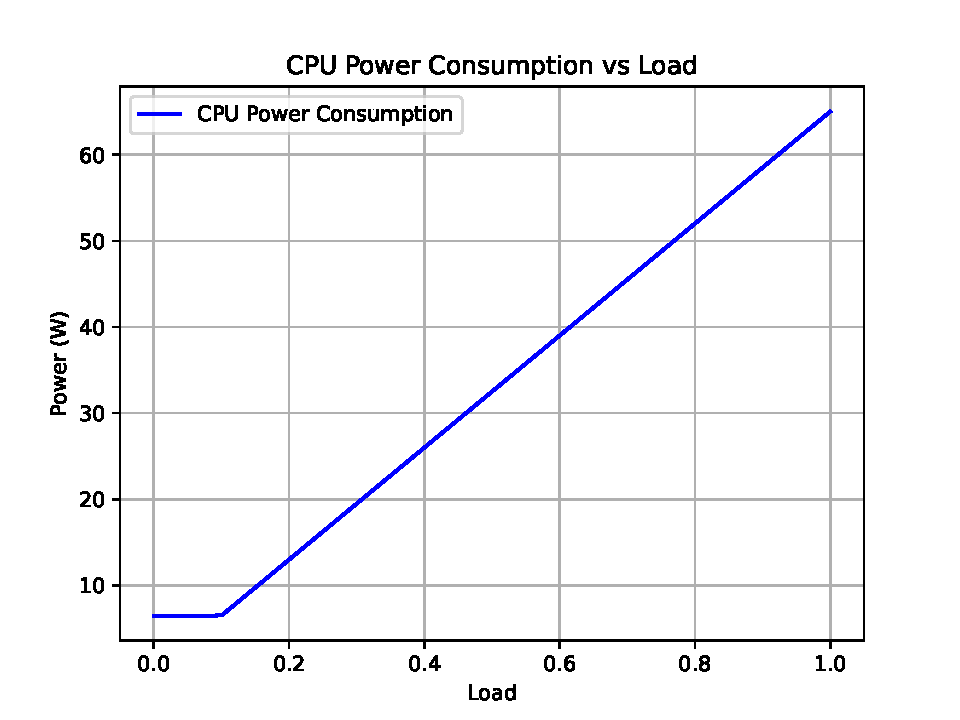
\includegraphics[width=0.8\linewidth]{img/CPU_power.pdf}
	\caption{Power consumption of the CPU}
	\label{fig:CPU_power}
\end{figure}
\subsection{RAM}
A slot of RAM consumes about $2-5W$ while being used, when in sleep mode it drops at $1 W$.
\subsection{GPU}
The power consumption of a GPU is more complex to compute but can be estimated by using the same formula as the CPU:
\begin{equation}
	Power = TDP \times \max(0.1, \text{load})
\end{equation}
\section{Reducing power consumption}
\subsection{Understanding the factors}
The power consumption of a component is the sum of two sources:
\begin{itemize}
	\item Static power: Minimum power consumed to keep the component on plus tiny leaks. High voltage induce more leaks.
	\item Dynamic power: Power consumed due to the activity, it's given by the formula:
	\begin{equation}
		P = C V^2 A f
	\end{equation}
	where $C$ is the capacitance, $V$ is the voltage, $A$ is the activity factor (number of switches of transistors per clock cycle) and $f$ is the frequency.\\
\end{itemize}
High frequency induce high voltage. Which leads us to the concept of Dynamic voltage and frequency scaling (DVFS). This technique allows to reduce the power consumption of !!a component by reducing the voltage and frequency when we doesn't need it. Thus we dynamically change voltage to adapt to the component load required. \\
\begin{itemize}
	\item [$\rightarrow$] NB: the performance of a program is affected only if it's compute-bounded not if it's bandwidth-bounded.
\end{itemize}
\subsection{Gating}
Gating is a way to save power when a CPU (or GPU) core is idle . The idea is to reduce or cut off power to unused parts of the chip in steps, depending on how long it’s been idle.
\begin{enumerate}
	\item \textbf{Clock gating}: Make some parts of the chip stop receiving clock signals (idle mode for them). 
	\item \textbf{Voltage Reduction (deeper idle)}: Reduce the voltage for the idle parts of the chip or the whole chip. 
	\item \textbf{Power Gating (deepest idle)}: The chip turns off parts of the circuit (cuts off the power supply entirely).
\end{enumerate}
\subsection{Reducing the power consumption of a program}
DVFS and gating are done automatically so how can we reduce the power consumption of a program? 
\begin{itemize}
	\item Limits the number of threads, especially if the program is bandwidth-bounded.
	\item Use shared memory instead of global memory to reduce the number of accesses to the global memory. It helps to improve the time of computing and the power efficiency.
	\item \textcolor{red}{TODO: Talk about warps and interleaving count}
\end{itemize}
\chapter{Useful tools}
\section{OpenMP}\label{OpenMP}
\textcolor{red}{TODO: Improve}\\
\textit{OpenMP} is a library that allows to parallelize code, it is better than \textit{lpthread} for multiple reasons:
\begin{itemize}
	\item Easy to add to an existing code, because of the compilation directives (\texttt{\#pragma omp}). It's an implicit gestion of the threads unlike \textit{lpthreads} that require an explicit gestion. It allows to parallelize a code without changing the whole structure of the code.
	\item Automatic gestion of the threads, for example if you want to parallelize a loop, you don't have to create the threads, the library will do it for you and optimize the number of threads.
	\item Simplified synchronization with tools. \textit{OpenMP} provides tools to synchronize the threads like \texttt{critical}, \texttt{atomic}, \texttt{barrier}, etc. They help to protect the shared data between the threads.
	\item Optimized use of the cache
	\item Compatible with \textit{SIMD}
	\item Portability: it is compatible with \textit{Windows}, \textit{Linux}, \textit{MacOS}. With multiple CPU architectures like \textit{Intel}, \textit{AMD}, \textit{ARM}, etc.
\end{itemize}
\section{Slurm}
\subsection{What is Slurm?}
\textbf{Slurm} stands for \textit{Simple Linux Utility for Resource Management}. It is an open-source job scheduler used in high-performance computing environments, such as university clusters or research supercomputers.
\subsection{How to use Slurm?}
\subsection{Slurm Topology}
\section{OpenCL}
\chapter{PAA - PDEs}
\section{Introduction}
Throughout this chapter, we will use the simple example of the diffusion equation. It is expressed as 
\begin{equation}
	\partial_t u(x,y,z,t) = \kappa \nabla^2 u(x,y,z,t) + f(t,x,y,z)
\end{equation}
To that, we add an initial condition and boundary conditions:
\begin{itemize}
	\item Initial condition: $u(0,x,y,z) = u_0(x,y,z)$;
	\item General boundary condition: $ n\cdot \nabla u=0$ on $\Omega$;
	\begin{itemize}
		\item Dirichlet boundary condition: $u(t,0)$ given for all $t\ge0$;
		\item Neumann boundary condition: $\partial_x(t,0)$ given for all $t\ge0$;
	\end{itemize}
\end{itemize}
This equation can represent the diffusion of heat, particles, pollutants, etc. It is derived from two basic laws of physics:
\begin{itemize}
	\item Fourier law for heat: $\vec q=-\kappa \nabla u$;
	\item Conservation law: $\partial_t u = -\partial_x \vec q$;
\end{itemize}
\section{Finite differences methods}
We will now consider more specifically the 1D case:
\begin{equation}
	u_t(t,x)=u_{xx}(t,x) \qquad x\in [0,1]\qquad t\ge 0
\end{equation}
with conditions 
\begin{equation}
	\begin{cases}
		u(t,0)=u(t,1) = 0 \quad \forall t\\
		u(0,x) = u^0(x)
	\end{cases}
\end{equation}
There is usually no analytical solution to the equation, and this is why we can use numerical method to find the solution. 
\subsection{The $\theta$-method}
In finite differences, we discretize the domain in a mesh, like displayed on figure \ref{fig:finite_diff}.
\begin{figure}[H]
	\centering
	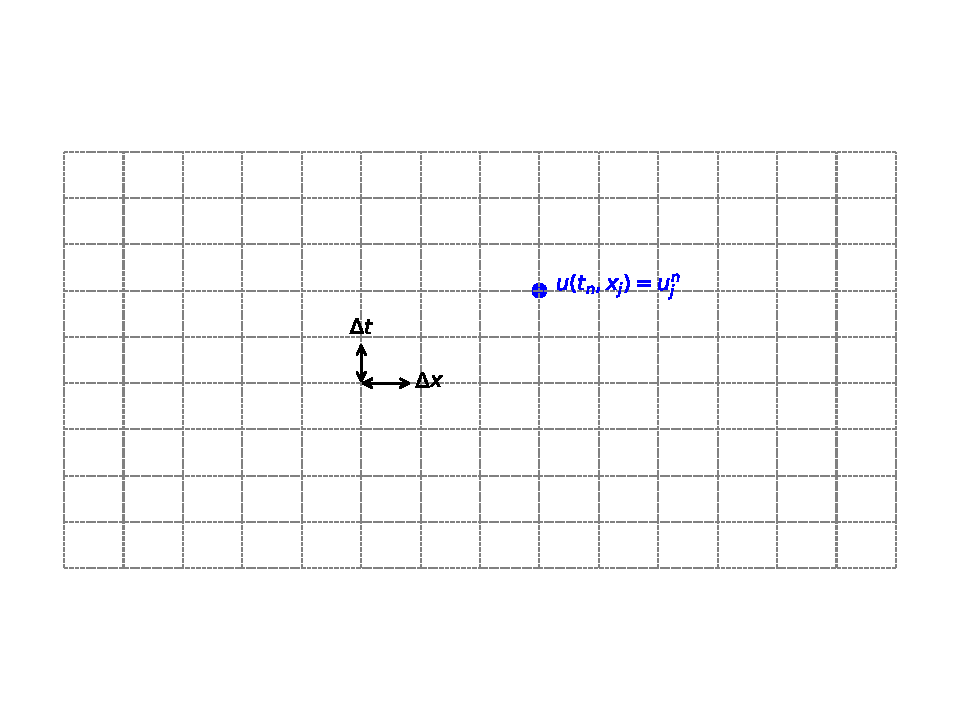
\includegraphics[width = .7\textwidth]{img/finite_diff.pdf}
	\caption{Discretization of the domain}
	\label{fig:finite_diff}
\end{figure}
The $\theta$-method consists in taking a linear combination of two approximations of the derivatives through finite differences:
\begin{equation}
	\frac{u_j^{n+1}-u_j^n}{\Delta t} = (1-\theta)\frac{u_{j+1}^n-2u_j^n+u_{j-1}^n}{\Delta x^2} + \theta \frac{u_{j+1}^{n+1}-2u_{j}^{n+1}+u_{j-1}^{n+1}}{\Delta x^2} + T_j^n
\end{equation}
Where $u_j^n$ denotes the exact value of the function $u(\cdot)$ at the given point, and $T_j^n$ is called the truncation error.\\
Using a truncation, i.e. using approximate values and deleting the truncation error term, the formula is 
\begin{equation}\label{eq:theta}
	\frac{U_j^{n+1}-U_j^n}{\Delta t} = (1-\theta)\frac{U_{j+1}^n-2U_j^n+U_{j-1}^n}{\Delta x^2} + \theta \frac{U_{j+1}^{n+1}-2U_{j}^{n+1}+U_{j-1}^{n+1}}{\Delta x^2}
\end{equation}
\subsection{Analysis principles of FD methods}
To be valid, a finite differences method needs to verify some basic principles:
\begin{itemize}
	\item Consistency along a refinement path: $T_j^n \xrightarrow{h\rightarrow 0} 0$;
\end{itemize}
\begin{figure}[H]
	\centering
	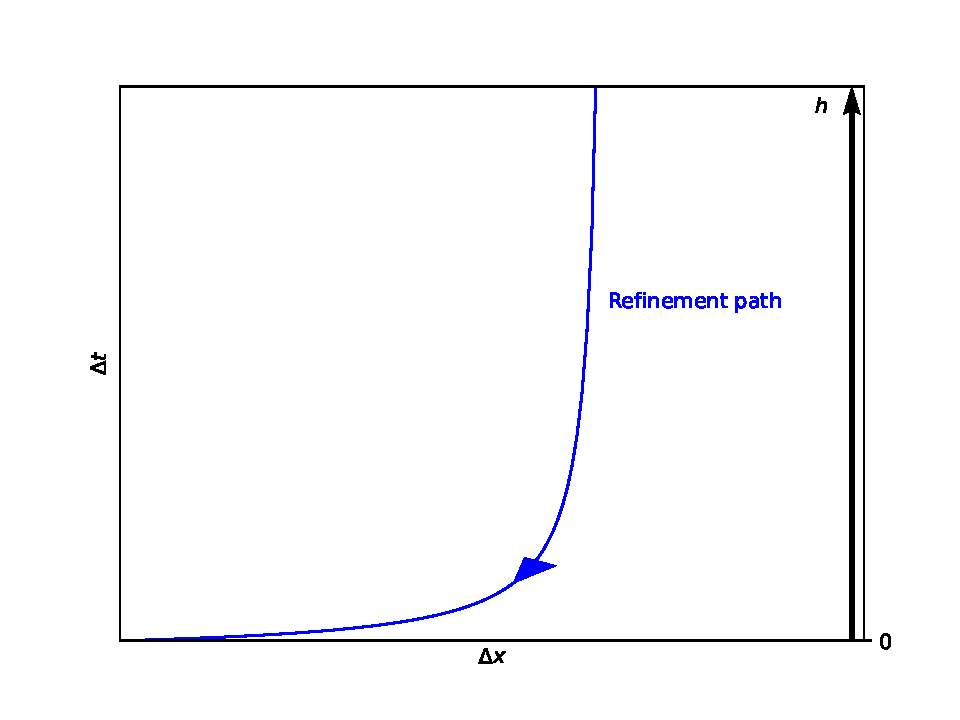
\includegraphics[width=.6\textwidth]{img/refinement.pdf}
\end{figure}
\begin{itemize}
	\item Accuracy: $|T_j^n| \le c (\Delta t^p + \Delta x^q)$, for all $\Delta t, \Delta x$ small, $c$ a constant and $p,q$ some accuracy parameters;
	\item Stability along a refinement path: For all solutions $v,w$ of the method and for all $t_F>0$, $\exists K_{t_F}$ such that $\| V^n - W^n \|\le K_{t_F} \|V^0 - W^0\|$ for all $n$ such that $n\Delta t\le t_F$, for $t_F$ the biggest time value;
	\item Lyapunov stability;
	\item Convergence along a refinement path: $U_j^n \xrightarrow{h\rightarrow 0}u(t,x)$ when $j\Delta x \rightarrow x$ and $n\Delta t \rightarrow t$. 
\end{itemize} 
\subsection{Value of $\theta$}
\subsubsection{$\theta=0$: FTCS (forward time, centered space)}
The formula becomes, when defining $\mu \coloneqq \kappa \Delta t/\Delta x^2$,
\begin{equation}
	U_j^{n+1} = \mu U_{j+1}^n + (1-2\mu)U_j^n + \mu U_{j-1}^n 
\end{equation}
\begin{figure}[H]
	\centering
	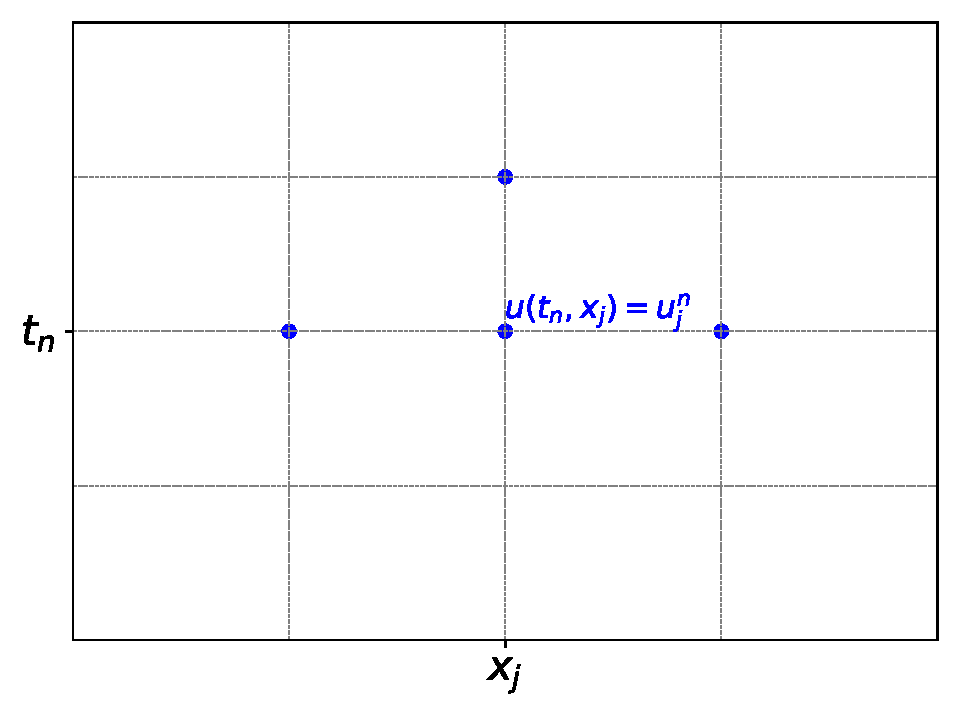
\includegraphics[width=.4\textwidth]{img/FTCS.pdf}
	\caption{Points used in the FTCS scheme.}
	\label{fig:FTCS}
\end{figure}
\subsubsection{$\theta=1$: BTCS (backward time, centered space)}
The formula becomes
\begin{equation}
	U_j^{n} = -\mu U_{j+1}^{n+1} + (1+2\mu)U_j^{n+1} - \mu U_{j-1}^{n+1} 
\end{equation}
\begin{figure}[H]
	\centering
	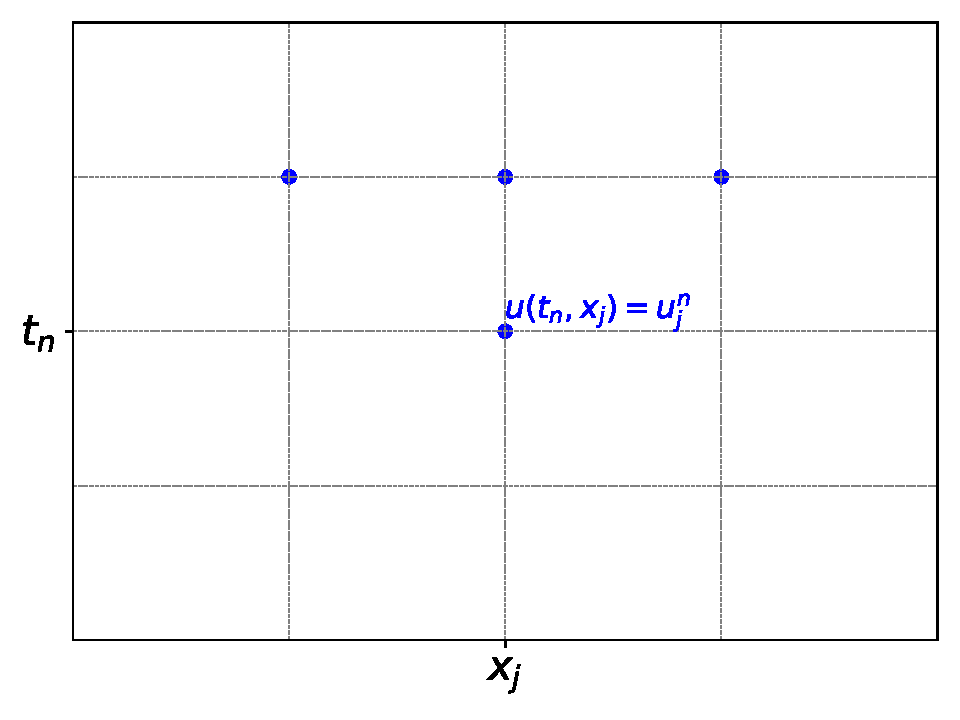
\includegraphics[width=.4\textwidth]{img/BTCS.pdf}
	\caption{Points used in the BTCS scheme.}
	\label{fig:BTCS}
\end{figure}
\subsubsection{$\theta=1/2$: Crank-Nicholson}
Crank Nicholson uses both the backward and forward time specifications. The formula is determined by replacing the value of $\theta$ but is tedious to write. The points it uses are displayed on figure \ref{fig:CN}
\begin{figure}[H]
	\centering
	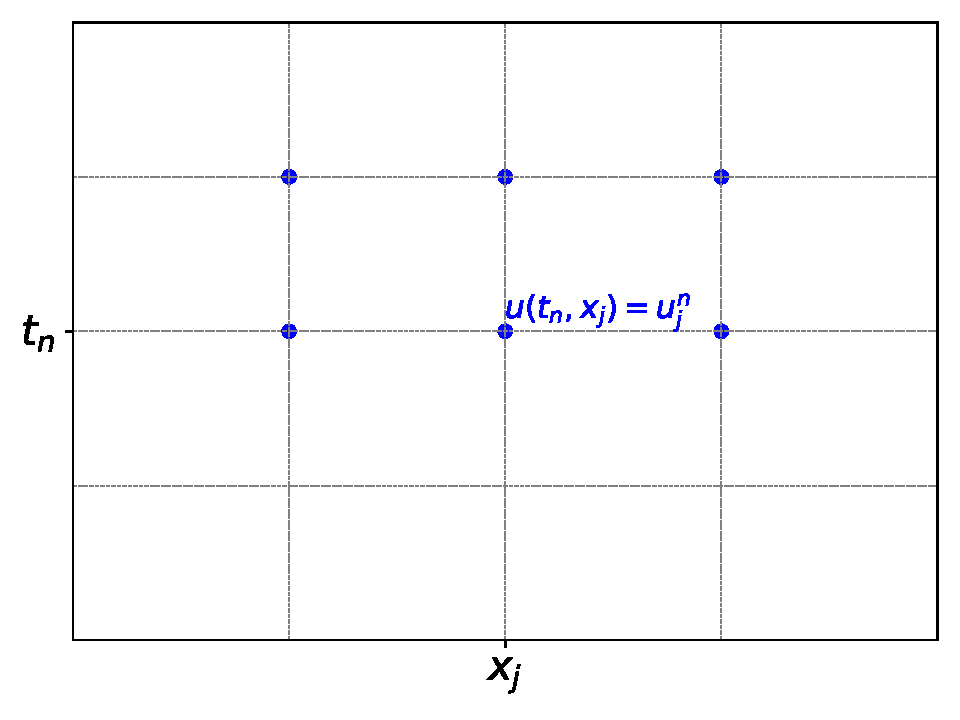
\includegraphics[width=.4\textwidth]{img/CN.pdf}
	\caption{Points used in the Crank-Nicholson scheme.}
	\label{fig:CN}
\end{figure}
\subsection{Truncation error}
By definition, the truncation error term is given by
\begin{equation}
	T^n_j = \frac{\delta_t u_j^{n+\frac{1}{2}}}{\Delta t} - \frac{\theta \delta_x^2u_j^{n+1} + (1-\theta)\delta_x^2u_j^n}{\Delta x^2}
\end{equation}
where we define $\delta_tu_j^{n+\frac{1}{2}}=u_j^{n+1}-u_j^n$ and $\delta_x^2u_j^n = u_{j+1}^n - 2 u_j^n + u_{j-1}^n$. Using a Taylor development series for each of the $u_j^n$, with reference point $(t_{n+\frac{1}{2}}, x_j)$, we can show that 
\begin{equation}
	T^n_j = \left(\left(\frac{1}{2}-\theta\right)\Delta t-\frac{1}{2}\Delta x^2\right) u_{xxxx} -\frac{1}{12}\Delta t^2u_{ttt} + \dots = \mathcal{O}(\Delta t, \Delta x^2)
\end{equation}
And for Crank-Nicholson, this becomes $\mathcal{O}(\Delta t^2, \Delta x^2)$. 
\subsection{Fourier stability analysis}
From equation \eqref{eq:theta}, we see that $U^{n+1}$ depends linearly in $U^n$ and we can make the guess that the solution will thus have the form 
\begin{equation}
	U_j^n = (\lambda(k))^n e^{ikj\Delta x} \qquad k\in \R
\end{equation}
Replacing in equation \eqref{eq:theta} and solving for $\lambda(k)$, we get
\begin{equation}
	\lambda(k) = \frac{1-4\mu(1-\theta)\sin^2\frac{k\Delta x}{2}}{1+4\mu \theta \sin^2 \frac{k\Delta x}{2}}
\end{equation}
By the discrete Fourier transform, every solution can be written 
\begin{equation}
	U_j^n = \sum_k c_k (\lambda(k))^n e^{ikj\Delta x}
\end{equation}
We know that, if $|\lambda(k)| \le 1$ for all $k$, then the $\theta$-scheme is Lyapunov stable. This condition is equivalent to 
\begin{equation}
	\mu(1-2\theta) \le \frac{1}{2}
\end{equation}
\begin{itemize}
	\item [$\to$] Note: this property is sufficient but not necessary. 
\end{itemize}
Let us now define the matrix 
\begin{equation}
	C(\beta) = \begin{bmatrix}
		1-2\beta & \beta & \ddots\\
		\beta & 1-2\beta & \beta & \ddots \\
		0 & \beta & 1-2\beta & \beta \\
		& & \ddots & \ddots & \ddots \\
		& & \beta & 1-2\beta & \beta \\
		& & & \beta & 1-2\beta \\ 
	\end{bmatrix} \in \R^{J-1 \times J-1}
\end{equation}
The $\theta$-scheme can be written in matrix form:
\begin{equation}
	\underbrace{C(-\mu \theta)}_{\eqqcolon B_1}U^{n+1} = \underbrace{C(\mu(1-\theta))}_{\eqqcolon B_0} U^n \Longleftrightarrow U^{n+1} = \underbrace{(C(-\mu\theta))^{-1} C(\mu(1-\theta))}_{=B_1^{-1}B_0 \eqqcolon A} U^n
\end{equation}
We can show that the eigenvalues of $C(\beta)$ and their corresponding eigenvectors are 
\begin{equation}
	v_\ell = 1-4\beta \sin^2 \frac{\pi \ell}{2J} \qquad x_\ell = \begin{bmatrix}
		\sin\frac{\pi \ell}{J} \\ \vdots \\ \sin \frac{\pi \ell(J-1)}{J}
	\end{bmatrix} \qquad  \ell=1,\dots, J-1 
\end{equation}
Hence the eigenvalues of the matrix $A$ are 
\begin{equation}
	v_ell = \frac{1-4\mu(1-\theta) \sin^2\frac{\pi \ell}{2J}}{1+4\mu\theta \sin^2 \frac{\pi \ell}{2J}} \qquad \ell = 1,\dots,J-1
\end{equation}
Their module must be smaller than 1 for the system to be Lyapunov stable (for all $\ell= 1,\dots,J-1$). This is equivalent to the condition 
\begin{equation}
	\frac{1-4\mu(1-\theta) \sin^2\frac{\pi (J-1)}{2J}}{1+4\mu\theta \sin^2 \frac{\pi (J-1)}{2J}} \ge -1
\end{equation}
\subsection{Dufort-Frankel scheme}
\begin{equation}
	U_j^{n+1} = U_j^{n-1} + 2\mu \left(U_{j-1}^n + U_{j+1}^n - U_j^{n+1}-U_j^{n-1}\right)
\end{equation}
\begin{figure}[H]
	\centering
	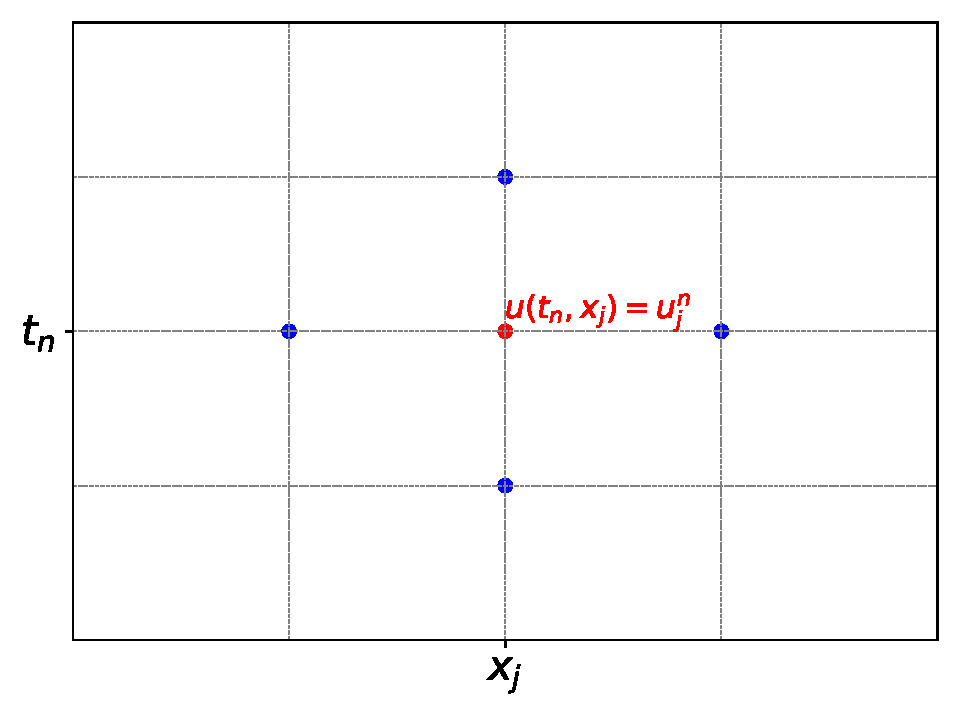
\includegraphics[width = .4\textwidth]{img/DF.pdf}
\end{figure}
Let us analyse the stability, given a solution of the form $U_j^n = \lambda^n e^{ikj\Delta x}$, which gives us the values
\begin{equation}
	\lambda_\pm = \frac{2\mu \cos(k\Delta x) \pm \sqrt{1-4\mu^2\sin^2(k\Delta x)}}{1+2\mu}
\end{equation}
We can show through the analysis of the $\lambda$ that this method is unconditionnaly stable, but not unconditionnaly consistent. 
\begin{itemize}
	\item [$\to$] Note: a scheme taking Dufort-Frankel with the additional point $(t_n, x_j)$ is unconditionnally unstable. 
\end{itemize}
\section{Finite volume methods}
Let us study the Poisson equation, written in the following form
\begin{equation}
	\nabla \cdot (\kappa(x)\nabla u) = f \quad \text{   in   }\quad  \Omega \subseteq \R^n
\end{equation}
\subsection{Voronoi cells}
The idea of finite volumes consists in creating cells given some vertices $\{x_i\}_i \subset \Omega$. The Voronoi cells are defined as 
\begin{equation}
	V_i = \{x\in \Omega:\ \|x-x_i\| \le \|x-x_j\| ,\ \forall j\neq i\}
\end{equation}
\begin{figure}[H]
	\centering
	
\includegraphics[width = .5\textwidth]{img/voronoi.png}
	\caption{Voronoi cells.}
	\label{fig:voronoi}
\end{figure}
The method is the following: by integrating over each cell, we can then use the divergence theorem to approximate using finite differences. 
\begin{equation}
	\begin{aligned}
		\int_{V_i} \nabla \cdot (\kappa(x)\nabla u)dx &= \int_{V_i} fdx \\
		\int_{\partial V_i}\kappa(x)\nabla u\cdot n ds&\approx f_i Vol(V_i)\\
		\sum_{j\sim i}K_{ij}\frac{u_j-u_i}{\underbrace{\|x_j-x_i\|}_{\eqqcolon h_{ij}}} \ell_{ij} \approx f_i Vol(V_i)
	\end{aligned}
\end{equation}
where the notation $j\sim i$ denotes the neighbours $j$ of point $i$, $K_{ij} = \kappa \left(\frac{x_i+x_j}{2}\right)$, $\ell_{ij}$ is the length of the interface between cells $i$ and $j$. This gives the finite volume scheme:
\begin{equation}
	\sum_{j\sim i} K_{ij} \frac{U_j-U_i}{h_{ij}} \ell_{ij} = Vol(V_i)f_i \qquad \forall i
\end{equation}
\subsection{Boundary conditions}
\begin{itemize}
	\item Dirichlet: if the condition is $u(x)=g(x)$ $\forall x\in \partial \Omega$, we write for points $x_k$ on the boundary $U_k = g(x_k)$;
	\item Neumann: the condition is $\nabla u\cdot n = g$ on $\partial \Omega$ and we use it in the form \[\int_{\partial V_i}\kappa(x)\nabla u\cdot n ds \approx \sum_j K_{ij}\frac{u_j-u_i}{h_{ij}}\ell_{ij} + \int_p \kappa(x)\nabla u\cdot nds,\] where $p$ is the boundary of cell $V_i$, and the integral can be approximated by quadrature.
\end{itemize}
\subsection{Analysis of principles}
The analysis of principles is complicated using finite volumes. However, here are the results:
\begin{itemize}
	\item Consistency: finite volume schemes are not consistent in general;
	\item Convergence: yes;
\end{itemize}
\section{Summary}
\begin{center}
	\begin{table}[ht]
		\centering
		\begin{tabularx}{\textwidth}{|X|X|X|}
			\hline
			&+ & - \\ \hline \hline
			Finite differences & Easy to understand and program & Cumbersome for non-rectangular domains or non-Dirichlet boundary conditions \\ \hline
			Finite volumes & Works for arbitrary geometries and meshes & Higher order methods are difficult to obtain \\ \hline
			Finite elements & Works for arbitrary geometries and meshes; & More complicated to implement \\
			& Higher order methods exist & \\ \hline
		\end{tabularx}
		\caption{Comparison of numerical methods.}
		\label{tab:comparison}
	\end{table}
\end{center}
\section{Hyperbolic equations in 1 space dimension}
\subsection{Linear advection equation}
\begin{equation}
	u_t + au_x = 0 \qquad u(x,t)=u^0(x)
\end{equation}
\subsection{CFL condition}
Consider the finite differences scheme:
\begin{equation}
	\frac{U_j^{n+1}-U_j^n}{\Delta t} + a \frac{U_j^n-U_{j-1}^n}{\Delta x} = 0
\end{equation}
which can also be written 
\begin{equation}
	U_j^{n+1} = (1-\nu)U_j^n + \nu_{j-1}^n\qquad \nu \coloneqq \frac{a\Delta t}{\Delta x}
\end{equation}
The CFL condition states that $\nu$ must be smaller than 1. If the scheme is convergent, then the condition holds. The meaning of the CFL condition is that the domain of dependence of the PDE, i.e. all the points that depend on $U_j^n$, is a subset of the domain of dependence of the numerical scheme. 
\end{document}